\documentclass[10pt,twocolumn,letterpaper]{article}

\usepackage[utf8]{inputenc}
\usepackage[margin=0.75in]{geometry}
\usepackage{amsmath,amssymb,amsfonts}
\usepackage{graphicx}
\usepackage{booktabs}
\usepackage{multirow}
\usepackage{subcaption}
\usepackage{dblfloatfix}
\usepackage{float}
\usepackage{balance}
\usepackage{hyperref}
\usepackage{xcolor}
\usepackage{microtype}
\usepackage{cite}
\usepackage[font=small,labelfont=bf,tableposition=top]{caption}

\hypersetup{
    colorlinks=true,
    linkcolor=blue!70!black,
    citecolor=green!50!black,
    urlcolor=magenta!70!black
}

\setcounter{topnumber}{4}
\setcounter{bottomnumber}{4}
\setcounter{totalnumber}{8}
\setcounter{dbltopnumber}{4}
\renewcommand{\topfraction}{0.95}
\renewcommand{\bottomfraction}{0.90}
\renewcommand{\textfraction}{0.05}
\renewcommand{\floatpagefraction}{0.75}
\renewcommand{\dbltopfraction}{0.95}
\renewcommand{\dblfloatpagefraction}{0.75}

\title{\textbf{Human Preference Alignment for Two-Stage Scene Graph Generation:\\YOLO12m-REACT++ on Panoptic Scene Graphs}}

\author{
    \textbf{Final Internship Report} \\
    Vision \& Language Navigation Team, VinRobotics \\
    Quoc Anh Phan \\
    {\small\texttt{pqa1085@gmail.com}}
}

\date{\today}

\begin{document}

\maketitle

\begin{abstract}
Scene Graph Generation (SGG) represents an image as objects and directed semantic relations. This report integrates and evaluates learning from human preference for a two-stage SGG system on the Panoptic Scene Graph (PSG) benchmark. The pipeline uses a frozen GeneralizedYOLO/YOLO12m detector as Stage~1 and aligns the REACT++ relation classifier in Stage~2 from pairwise human choices over uncertain predicate candidates. To collect these choices, we build a GUI application that displays detected subject-object pairs, the image overlay, and two competing predicate hypotheses selected by an uncertainty-identification module. The training objective combines a Bradley-Terry preference loss with masked KL retention and prototype anchoring to reduce catastrophic semantic drift during preference fine-tuning. PSG test evaluation shows that adding preference learning to the two-stage model improves relation quality over the original baseline: SGDet mR@50 increases from $26.37\%$ to $26.95\%$ and F1@50 from $31.22\%$ to $31.58\%$, while bbox mAP remains unchanged at $56.57\%$. Ablation studies show that preference loss alone overfits the collected choices and damages the broader predicate distribution, whereas the full RLHP objective preserves relation-space stability.
\end{abstract}

\section{Introduction}
\label{sec:intro}

Scene Graph Generation (SGG) parses an image into a directed graph $\mathcal{G}=(\mathcal{V},\mathcal{E})$, where nodes correspond to localized objects and edges correspond to predicates in triplets $(s,p,o)$~\cite{krishna2017visual,yang2022psg}. Such graphs are useful for downstream vision-language reasoning because they expose an intermediate symbolic structure instead of only dense visual features.

The practical bottleneck is predicate quality. Modern SGG models often localize salient objects reliably but collapse ambiguous relations into generic predicates such as \textit{on}, \textit{of}, \textit{near}, or \textit{with}. This is especially harmful for long-tail predicates, where a small semantic change can determine whether a graph is useful for navigation or reasoning. Section~\ref{sec:results} investigates how preference alignment directly addresses these ambiguities both quantitatively and qualitatively.

This report focuses on a practical learning-from-human-preference workflow for a two-stage YOLO12m-REACT++ SGG pipeline~\cite{neau2024reactpp}. Stage~1 performs object detection with a frozen YOLO12m detector, while Stage~2 predicts predicates for directed object pairs with REACT++. The alignment target is therefore narrow by design: human feedback should modify relation classification without changing the detector or the object features that determine bbox mAP.

\paragraph{System focus.}
The work has three connected components. First, a GUI application is built to collect pairwise predicate preferences from PSG train images. Second, an uncertainty-identification module chooses informative subject-object pairs by comparing the top two foreground predicate hypotheses, so annotators spend time on ambiguous but model-relevant relations. Third, the preference-training objective is evaluated with ablations on auxiliary retention losses, because a small preference dataset can improve the queried pairs while still causing catastrophic drift across unlabelled predicates.

\paragraph{Goals.}
The report has three goals:
\begin{enumerate}
    \item build a GUI application and uncertainty selector for collecting reliable human predicate preferences on PSG train images;
    \item integrate preference learning into the two-stage YOLO12m-REACT++ pipeline while keeping Stage~1 detection frozen;
    \item evaluate PSG test performance and ablate masked KL retention and prototype anchor losses as safeguards against catastrophic drift.
\end{enumerate}

\paragraph{Outline.}
Section~\ref{sec:methodology} describes the two-stage architecture, uncertainty identification, GUI, and audit pipeline. Section~\ref{sec:rlhp} formalizes preference learning and retention. Section~\ref{sec:experiments} gives datasets, metrics, and settings. Section~\ref{sec:results} analyzes the preference data, training diagnostics, quantitative benchmark results, ablations, and qualitative changes.

\section{Methodology}
\label{sec:methodology}

\subsection{Two-Stage YOLO12m-REACT++ Pipeline}

The model separates object detection from relation classification:
\begin{equation}
    I \rightarrow \mathcal{B}=\{(b_i,c_i,\mathbf{f}_i)\}_{i=1}^{N}
    \rightarrow \{r_{ij,k}\}_{(i,j),k}.
\end{equation}
Stage~1 uses GeneralizedYOLO with a YOLO12m backbone to produce boxes, object labels, object confidences, and RoI features. During preference training, all detector, object-path, and relation-encoder parameters remain frozen. This is the main architectural reason bbox mAP stays invariant.

Stage~2 uses REACT++ to compose directed subject-object representations. For each directed pair $(i,j)$, REACT++ combines subject and object features, object semantics, geometry, and scene context tokens. The relation representation $\mathbf{z}_{ij}$ and predicate prototypes $\mathbf{P}_k$ are projected into a shared normalized space:
\begin{equation}
    \hat{\mathbf{z}}_{ij} =
    \frac{\phi_{\mathrm{proj}}(\mathbf{z}_{ij})}
         {\|\phi_{\mathrm{proj}}(\mathbf{z}_{ij})\|_2},
    \qquad
    \hat{\mathbf{p}}_k =
    \frac{\phi_{\mathrm{proj}}(\mathbf{P}_k)}
         {\|\phi_{\mathrm{proj}}(\mathbf{P}_k)\|_2}.
\end{equation}
The reward used by preference learning is the pre-softmax relation logit:
\begin{equation}
    r_{ij,k} = \exp(s)\langle \hat{\mathbf{z}}_{ij},\hat{\mathbf{p}}_k\rangle,
    \label{eq:logits}
\end{equation}
where $s$ is REACT++'s learnable logit scale parameter. In the final alignment stage, trainable parameters are strictly restricted to the relation projection head $\phi_{\mathrm{proj}}$ and the logit scale $s$, while all object detector components and relation feature representations remain completely frozen.

\subsection{Uncertainty Identification}
\label{sec:uncertainty}

The annotation tool should not ask users to label arbitrary relations. It first filters objects by confidence and maximum count, creates all directed pairs, and extracts each relation's top two foreground predicates. The selector then:
\begin{enumerate}
    \item keeps a Top-K shortlist by highest top predicate probability $p_1$;
    \item selects Top-M relations inside that shortlist by the smallest relative margin
    \begin{equation}
        \Delta_{\mathrm{rel}} = \frac{p_1-p_2}{p_1+p_2};
    \end{equation}
    \item presents the two predicates in shuffled order to avoid button-position bias.
\end{enumerate}
In empirical evaluation, the uncertainty-priority selector achieves a substantially higher mean uncertainty score than highest-probability sampling ($0.476$ vs. $0.223$) while consistently retaining confident candidate relations. Table~\ref{tab:selection_comparison} contrasts the selected examples.

\begin{table}[t]
\centering
\footnotesize
\caption{\textbf{Selection comparison.} Uncertainty-priority selection keeps high-confidence relations but favors pairs whose top two predicates are close, producing more informative queries than ranking only by $p_1$.}
\label{tab:selection_comparison}
\setlength{\tabcolsep}{2.2pt}
\resizebox{\columnwidth}{!}{%
\begin{tabular}{lllcrc}
\toprule
\textbf{Method} & \textbf{\#} & \textbf{Relation} & \textbf{Top Predicates} & \textbf{$p_1$} & \textbf{Uncertainty} \\
\midrule
Top prob. & 1 & person $\rightarrow$ skis & playing / wearing & 2.6\% & 86.1\% \\
Top prob. & 2 & skis $\rightarrow$ snow & on / in & 2.5\% & 6.7\% \\
Top prob. & 3 & person $\rightarrow$ snow & going down / standing on & 2.4\% & 16.1\% \\
\midrule
Uncertainty & 1 & person $\rightarrow$ skis & playing / wearing & 2.6\% & 86.1\% \\
Uncertainty & 2 & person $\rightarrow$ skis & standing on / playing & 0.4\% & 79.5\% \\
Uncertainty & 3 & person $\rightarrow$ snow & going down / walking on & 1.1\% & 45.3\% \\
\bottomrule
\end{tabular}%
}
\end{table}

Table~\ref{tab:selection_comparison} shows that relative-margin uncertainty prioritizes ambiguous predicate pairs while still keeping the relation candidates sufficiently confident. This focuses the human annotation budget on pairs where feedback is most informative for refining the model's decision boundaries.

\subsection{Feedback Encoding and Audit}

Figure~\ref{fig:feedback_collection} illustrates the graphical user interface developed to present detected subject-object bounding boxes and collect human preferences between candidate predicates. The GUI supports strong preference for either predicate, neutral preference (tie), no relation / both wrong, and undo. Strong preferences are encoded as one-hot target vectors $[1,0]$ or $[0,1]$, neutral preferences as $[0.5,0.5]$, and both-wrong labels as $[0,0]$. The pairwise preference optimization utilizes strong and neutral labels. Both-wrong samples are retained for dataset auditing and error analysis, but excluded from gradient optimization because they indicate false candidate hypotheses rather than a relative preference.

\begin{figure}[t]
    \centering
    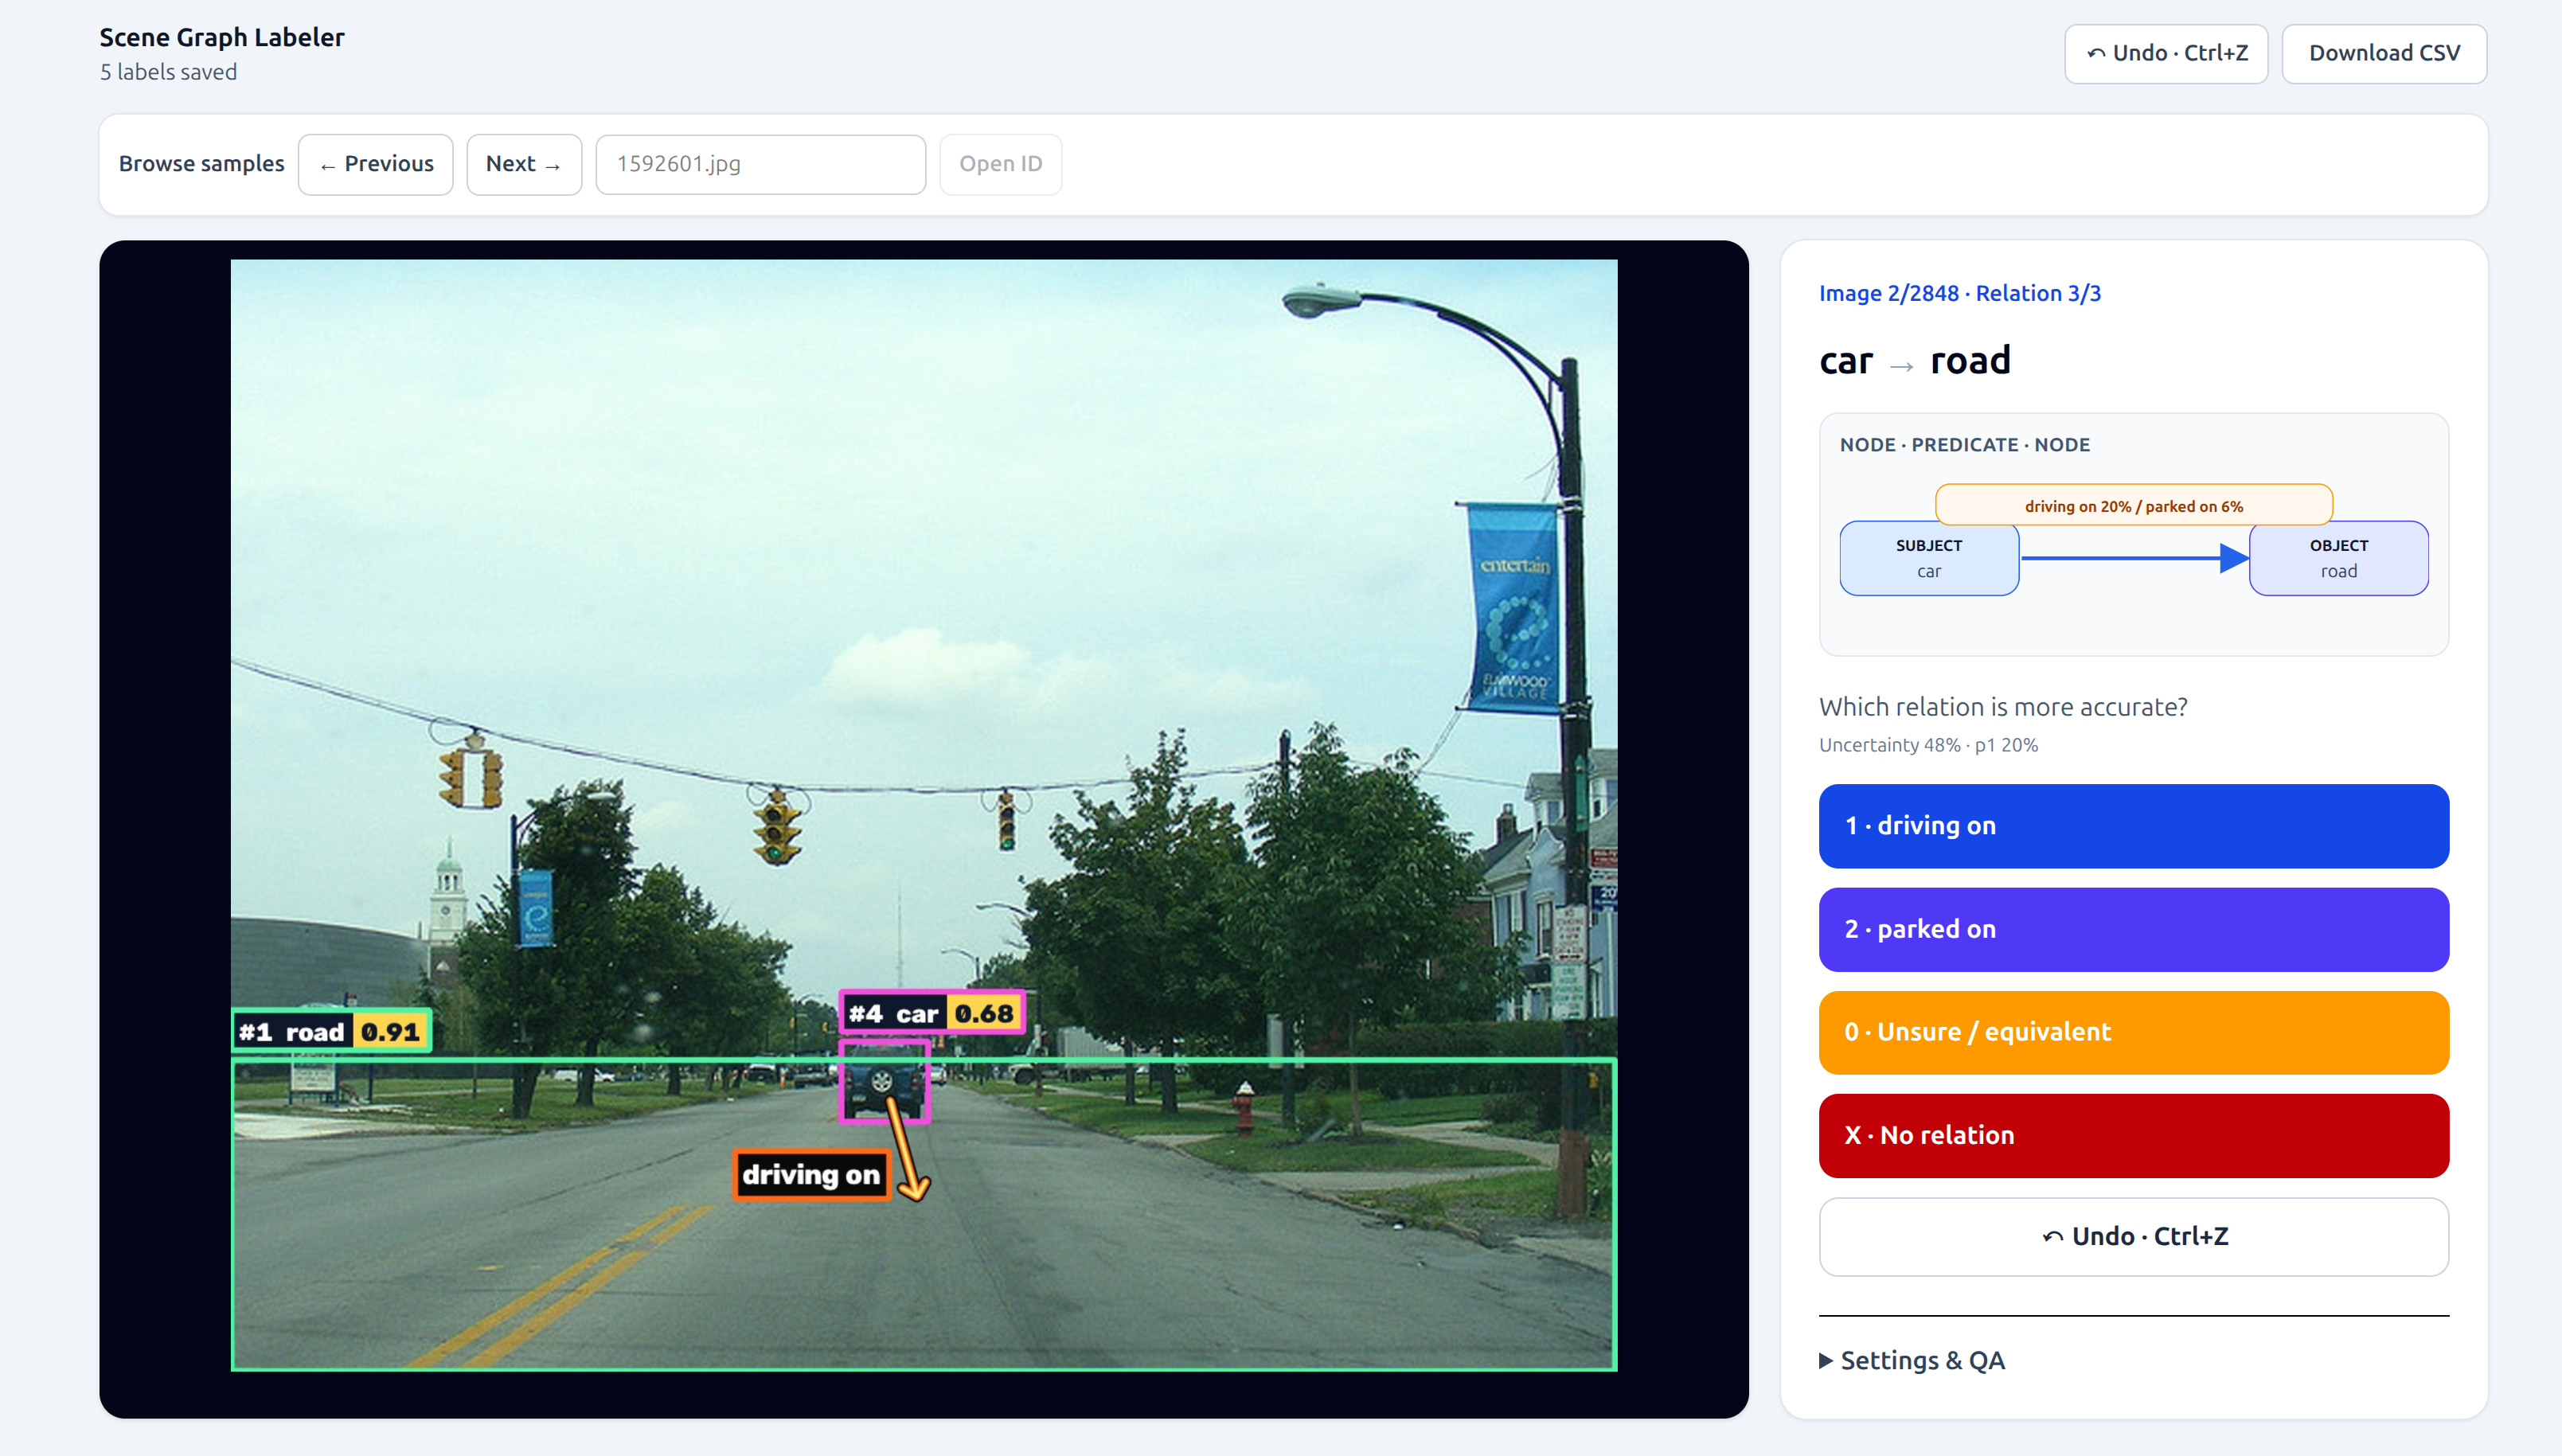
\includegraphics[width=\columnwidth]{figures/GUI_image.png}
    \caption{\textbf{Preference collection GUI.} The interface displays the image overlay, localized subject-object bounding boxes, and two candidate predicates for pairwise human feedback.}
    \label{fig:feedback_collection}
\end{figure}

Each saved answer includes image checksum, model/configuration/label-map SHA256, subject/object boxes and labels, both predicate IDs, the full relation distribution, and the displayed order. Before training, the audit pipeline verifies that no PSG test image appears in the preference set, re-matches subject/object predictions with category IDs and IoU $\ge 0.8$, aggregates duplicate votes, and splits the collected PSG-train feedback into internal training and validation subsets by image checksum. The final audited set contains $510$ raw feedback records over $168$ unique PSG train images: $376$ usable preference samples ($283$ train, $93$ validation) and $134$ audit-only both-wrong records. Pair matching and model-backed matching both reached $100\%$.

\section{Preference Learning Objective}
\label{sec:rlhp}

\subsection{Bradley-Terry Preference Loss}

Each preference annotation sample is indexed by $m = (I_m, s_m, o_m, p_{m,a}, p_{m,b}) \in \mathcal{D}_{\mathrm{pref}}$, where $I_m$ denotes the input image, $s_m$ and $o_m$ represent the localized subject and object bounding boxes, and $p_{m,a}, p_{m,b} \in \{1, \dots, C_{\mathrm{rel}}\}$ are the two candidate predicate categories displayed to the annotator.

Let $r_{m,a}$ and $r_{m,b} \in \mathbb{R}$ be the model's pre-softmax relation logits (computed via Eq.~\eqref{eq:logits}) for candidate predicates $p_{m,a}$ and $p_{m,b}$ on the directed pair $(s_m, o_m)$. Under the Bradley-Terry preference model parameterized with temperature scaling $\tau > 0$, the predicted probability $\pi_{m,k} = P(p_{m,k} \succ p_{m,\neg k} \mid I_m, s_m, o_m)$ that predicate $p_{m,k}$ ($k \in \{a, b\}$) is preferred over the alternative is given by:
\begin{equation}
    \pi_{m,k} = \frac{\exp(\tau r_{m,k})}{\exp(\tau r_{m,a}) + \exp(\tau r_{m,b})}.
    \label{eq:bt_prob}
\end{equation}
Here, $\tau = 0.1$ is an inverse temperature hyperparameter that calibrates the sharpness of the reward distribution.

Human feedback for sample $m$ is represented by a soft target probability vector $\mathbf{y}_m = [y_{m,a}, y_{m,b}]^\top$ satisfying $y_{m,a}, y_{m,b} \ge 0$ and $y_{m,a} + y_{m,b} = 1$:
\begin{itemize}
    \item \textbf{Strict preference ($p_{m,a} \succ p_{m,b}$):} $\mathbf{y}_m = [1, 0]^\top$;
    \item \textbf{Strict preference ($p_{m,b} \succ p_{m,a}$):} $\mathbf{y}_m = [0, 1]^\top$;
    \item \textbf{Neutral / Tie ($p_{m,a} \sim p_{m,b}$):} $\mathbf{y}_m = [0.5, 0.5]^\top$.
\end{itemize}

For a single sample $m$, the preference objective is formulated as the cross-entropy between the human preference distribution $\mathbf{y}_m$ and the model predicted choice probabilities $\boldsymbol{\pi}_m = [\pi_{m,a}, \pi_{m,b}]^\top$:
\begin{equation}
    \ell_{\mathrm{pref}}(m) = -\sum_{k\in\{a,b\}} y_{m,k} \log \pi_{m,k}.
\end{equation}
For a strict choice where predicate $p_w$ is preferred over $p_l$ ($\mathbf{y}_m=[1,0]^\top$), this reduces to the classical Bradley-Terry negative log-likelihood:
\begin{equation}
    \ell_{\mathrm{BT}}(m) = -\log \sigma\big(\tau(r_{m,w} - r_{m,l})\big),
\end{equation}
where $\sigma(z) = 1/(1+e^{-z})$ is the logistic sigmoid function.

Over a training batch of $M$ samples, the total preference loss is the weighted mean across all valid samples:
\begin{equation}
    \mathcal{L}_{\mathrm{pref}} = -\frac{\sum_{m=1}^M w_m \sum_{k\in\{a,b\}} y_{m,k}\log \pi_{m,k}}{\sum_{m=1}^M w_m},
    \label{eq:pref_loss}
\end{equation}
where $w_m \ge 1$ denotes the sample weight reflecting duplicate vote aggregation.

\subsection{Masked KL Retention Loss}

The preference loss $\mathcal{L}_{\mathrm{pref}}$ only constrains the relative order between the two candidate predicates $\{p_{m,a}, p_{m,b}\}$. Without explicit regularization, unconstrained optimization severely degrades performance on the remaining $55$ relation categories.

Let $C_{\mathrm{rel}} = 57$ denote the total number of relation classes in PSG (including background). For a given sample $m$, let $\mathbf{q}_m \in \Delta^{C_{\mathrm{rel}}-1}$ denote the full softmax output distribution produced by the current student model, and $\mathbf{q}_m^0 \in \Delta^{C_{\mathrm{rel}}-1}$ denote the baseline softmax distribution from the frozen teacher model. Let $\mathcal{O}_m = \{1, \dots, C_{\mathrm{rel}}\} \setminus \{p_{m,a}, p_{m,b}\}$ be the subset of all unlabelled predicate classes.

To preserve the teacher's knowledge outside the labelled pair, we decompose the distribution into the total unlabelled probability mass and the renormalized conditional distribution over $\mathcal{O}_m$:
\begin{align}
    M_m^0 &= \sum_{c\in\mathcal{O}_m} q_{m,c}^0, & M_m &= \sum_{c\in\mathcal{O}_m} q_{m,c}, \\
    \bar{q}_{m,c}^0 &= \frac{q_{m,c}^0}{M_m^0}, & \bar{q}_{m,c} &= \frac{q_{m,c}}{M_m} \quad (\forall c \in \mathcal{O}_m).
\end{align}
Here, $M_m^0$ and $M_m$ represent the total mass allocated to unlabelled categories, while $1 - M_m^0$ and $1 - M_m$ represent the aggregate mass of the candidate pair $\{p_{m,a}, p_{m,b}\}$. 

By the chain rule of Kullback-Leibler (KL) divergence, the masked retention loss per sample $m$ is decomposed into a total-mass divergence and a conditional divergence over unlabelled classes:
\begin{equation}
    \ell_{\mathrm{KL}}(m) = D_{\mathrm{KL}}^{\mathrm{mass}}(m) + M_m^0 \cdot D_{\mathrm{KL}}^{\mathrm{cond}}(m),
\label{eq:sample_kl}
\end{equation}
where:
\begin{align}
    D_{\mathrm{KL}}^{\mathrm{mass}}(m) &= M_m^0 \log \frac{M_m^0}{M_m} + (1-M_m^0) \log \frac{1-M_m^0}{1-M_m}, \\
    D_{\mathrm{KL}}^{\mathrm{cond}}(m) &= \sum_{c\in\mathcal{O}_m} \bar{q}_{m,c}^0 \log \frac{\bar{q}_{m,c}^0}{\bar{q}_{m,c}}.
\end{align}
The first term ensures that preference fine-tuning does not inflate or suppress the total probability volume assigned to non-target relations. The second term preserves the teacher's relative probability shape across all $55$ non-target predicates. Crucially, omitting the KL penalty within $\{p_{m,a}, p_{m,b}\}$ gives the model the necessary flexibility to adjust the relative logit ranking between the two queried predicates according to human feedback.

The weighted batch retention loss is computed as:
\begin{equation}
    \mathcal{L}_{\mathrm{KL}} = \frac{\sum_{m=1}^M w_m \ell_{\mathrm{KL}}(m)}{\sum_{m=1}^M w_m}.
    \label{eq:kl_loss}
\end{equation}

\subsection{Prototype Anchor Loss}

In REACT++, relation logits are computed via cosine similarity between visual relation representations and predicate prototypes (Eq.~\eqref{eq:logits}). Because only the projection head $\phi_{\mathrm{proj}}$ is trainable, updating it on a small preference dataset risks rotating the shared prototype manifold and distorting global semantic alignment.

To preserve the global semantic geometry, we anchor the normalized predicate prototypes $\hat{\mathbf{p}}_c$ to their frozen teacher counterparts $\hat{\mathbf{p}}_c^0$ via a cosine distance loss across all $C_{\mathrm{rel}}$ categories:
\begin{equation}
    \mathcal{L}_{\mathrm{proto}} = \frac{1}{C_{\mathrm{rel}}} \sum_{c=1}^{C_{\mathrm{rel}}} \left( 1 - \langle \hat{\mathbf{p}}_c, \hat{\mathbf{p}}_c^0 \rangle \right),
    \label{eq:proto_loss}
\end{equation}
where:
\begin{itemize}
    \item $\hat{\mathbf{p}}_c = \frac{\phi_{\mathrm{proj}}(\mathbf{P}_c)}{\|\phi_{\mathrm{proj}}(\mathbf{P}_c)\|_2} \in \mathbb{R}^d$ is the $\ell_2$-normalized prototype vector for predicate class $c$ in the current model;
    \item $\hat{\mathbf{p}}_c^0 \in \mathbb{R}^d$ is the corresponding normalized prototype vector from the frozen baseline model (detached from the computation graph as a static target);
    \item $\langle \hat{\mathbf{p}}_c, \hat{\mathbf{p}}_c^0 \rangle$ is the dot product (cosine similarity) between the normalized prototype embeddings;
    \item $C_{\mathrm{rel}} = 57$ is the total number of relation classes in PSG.
\end{itemize}

\paragraph{Total objective.}
The combined optimization objective for the Full RLHP model is:
\begin{equation}
    \mathcal{L}_{\mathrm{total}} = \mathcal{L}_{\mathrm{pref}} + \lambda_{\mathrm{KL}}\mathcal{L}_{\mathrm{KL}} + \lambda_{\mathrm{proto}}\mathcal{L}_{\mathrm{proto}},
    \label{eq:total_loss}
\end{equation}
where $\lambda_{\mathrm{KL}} = 20$ balances the masked distribution retention, $\lambda_{\mathrm{proto}} = 20$ regulates prototype manifold stability, and $\tau = 0.1$ governs the Bradley-Terry temperature scaling.

\section{Experimental Setup}
\label{sec:experiments}

\subsection{Datasets and Metrics}

\textbf{Preference data.} Human feedback is collected from PSG train images only. The audit rejects test leakage before any training step. The final dataset has $510$ feedback rows, $376$ usable preference samples, and no dropped records; train/validation in this report refers to the internal preference split, not PSG validation images.

\textbf{Evaluation data.} The final comparison is run on the PSG test benchmark with $2,177$ images, $134$ object categories including background, and $57$ relation classes including background.

\textbf{Metrics.} The main benchmark setting is SGDet, where boxes, object labels, and predicates are all predicted. Let $\mathcal{G}_i$ be the ground-truth triplets for image $i$ and $\mathcal{P}^K_i$ the top-$K$ predicted triplets. Recall@K is:
\begin{equation}
    R@K = \frac{1}{N}\sum_{i=1}^{N}
    \frac{|\mathcal{G}_i \cap \mathcal{P}^K_i|}{|\mathcal{G}_i|}.
\end{equation}
For predicate class $c$, let $\mathcal{G}_{i,c}$ and $\mathcal{P}^K_{i,c}$ denote triplets of class $c$. Mean Recall@K averages class-wise recall:
\begin{equation}
    mR@K =
    \frac{1}{C}\sum_{c=1}^{C}
    \frac{\sum_i |\mathcal{G}_{i,c} \cap \mathcal{P}^K_{i,c}|}
         {\sum_i |\mathcal{G}_{i,c}|}.
\end{equation}
We report Recall@K (R@K), Mean Recall@K (mR@K), F1@K, and object detection bbox mAP. Mean Recall is especially emphasized as the primary evaluation metric because it measures macro-averaged performance across all relation classes without being skewed by head predicates.

\subsection{Training Settings}

Training uses AdamW, weight decay $0.01$, gradient accumulation over $4$ image groups, gradient clipping at norm $1.0$, and deterministic image-group shuffling. The best reported configuration, \textbf{Full RLHP}, uses learning rate $2\times10^{-6}$, $\tau=0.1$, $\lambda_{\mathrm{KL}}=20$, and $\lambda_{\mathrm{proto}}=20$ for $5$ epochs. Every candidate model is saved without overwriting the baseline; frozen parameter hashes are checked after training.

\section{Results and Discussion}
\label{sec:results}

\subsection{Preference Data Analysis}
\label{sec:pref_analysis}

% Figure 2 declared inside Section 5.1 as single-column stacked subfigures
\begin{figure*}[t]
    \centering
    \begin{subfigure}[b]{0.498\textwidth}
        \centering
        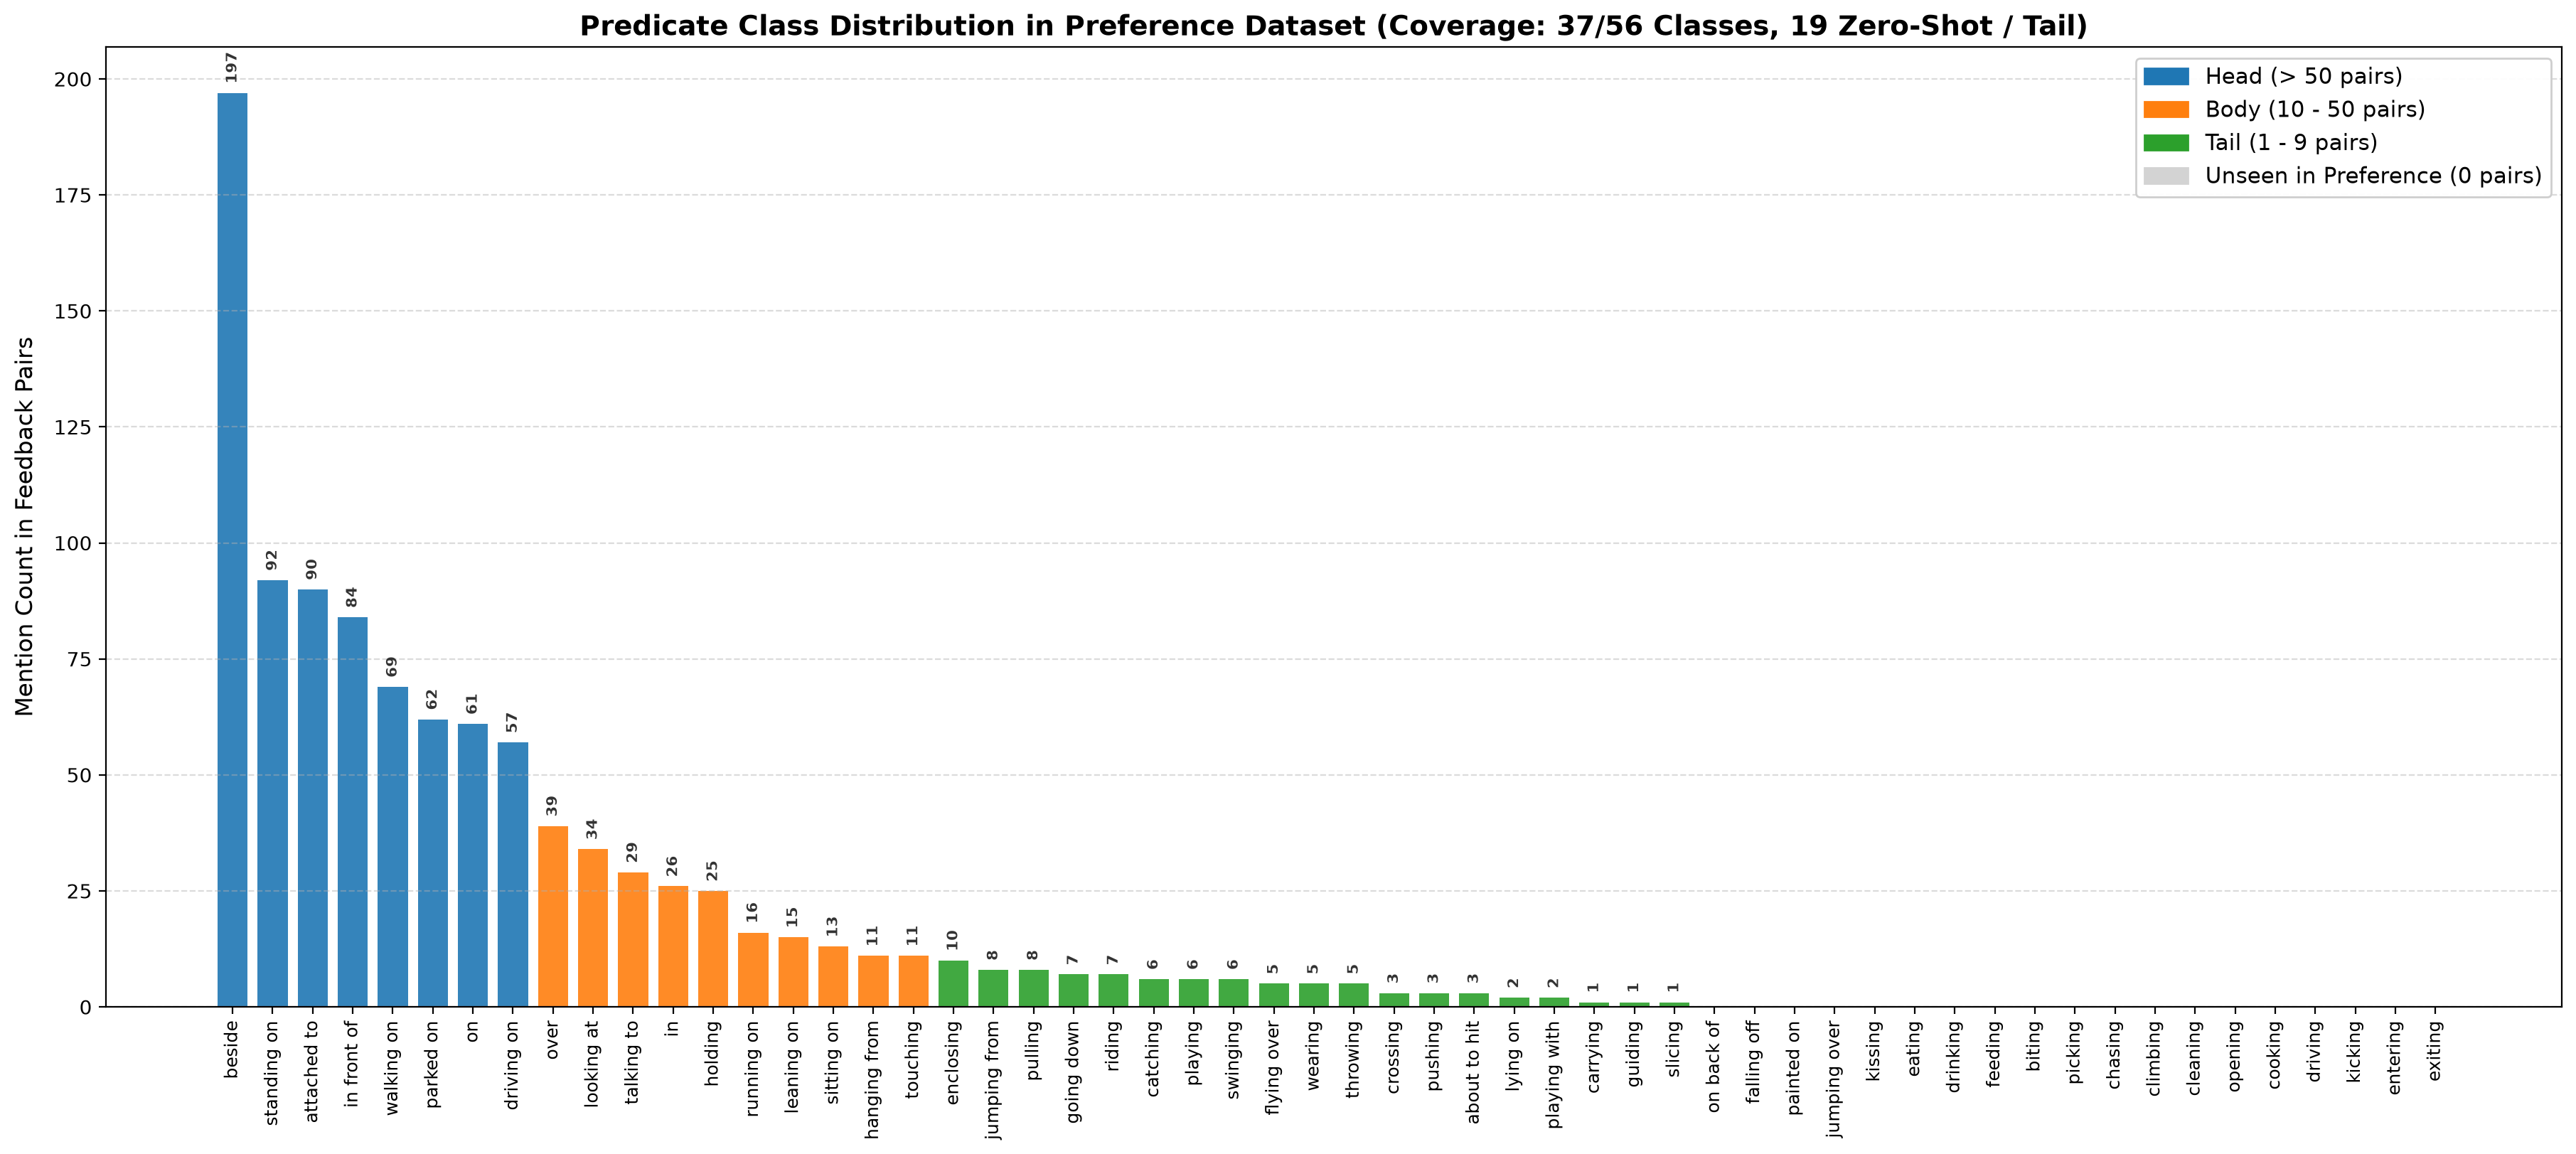
\includegraphics[width=\linewidth]{figures/preference_class_distribution.png}
        \caption{Preferred predicate distribution}
        \label{fig:preference_distribution}
    \end{subfigure}
    \hfill
    \begin{subfigure}[b]{0.498\textwidth}
        \centering
        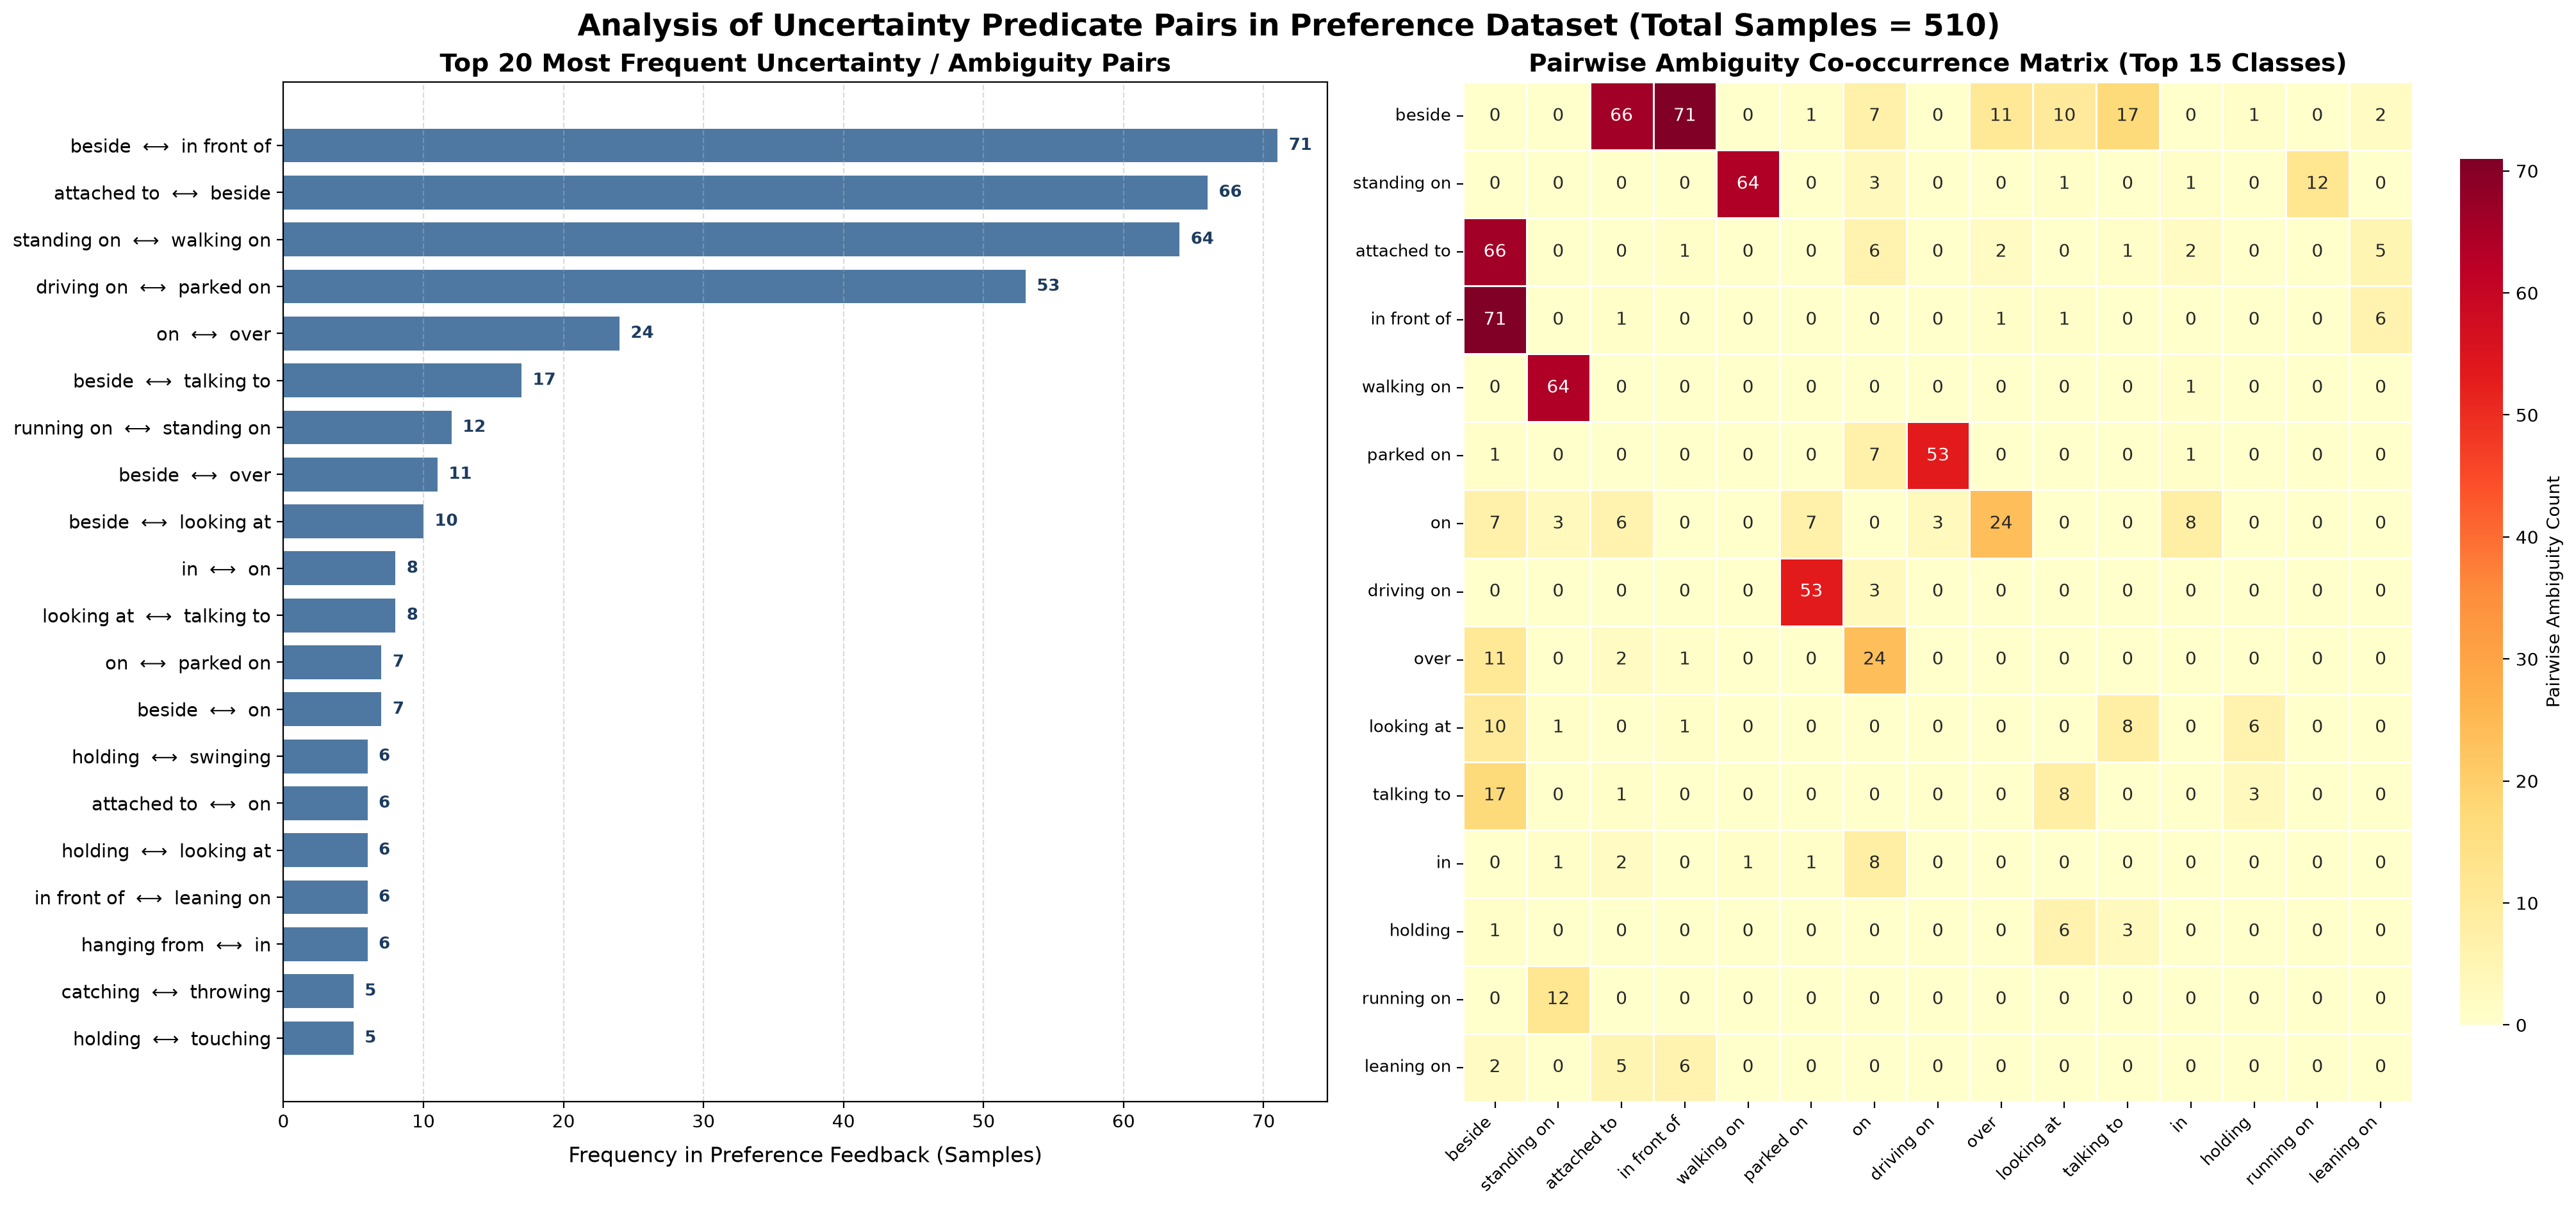
\includegraphics[width=\linewidth]{figures/uncertainty_pairs_distribution.png}
        \caption{Uncertain predicate pairs prioritized for annotation}
        \label{fig:pair_dist}
    \end{subfigure}
    \caption{\textbf{Preference data analysis.} (a) Distribution of preferred predicates after human feedback, showing concentration on frequent spatial/action relations. (b) Distribution of active uncertainty pairs, showing that prediction ambiguities primarily cluster in head and body relations.}
    \label{fig:pref_data_analysis}
\end{figure*}

Figure~\ref{fig:preference_distribution} presents the distribution of preferred predicates across all audited human feedback samples, while Figure~\ref{fig:pair_dist} details the distribution of uncertain candidate pairs prioritized by the uncertainty identification module.

\paragraph{Head and body ambiguity.}
A joint examination of Figures~\ref{fig:preference_distribution} and~\ref{fig:pair_dist} reveals a key operational characteristic of the two-stage SGG framework: the baseline model is not only intrinsically biased toward dominant predicate classes, but simultaneously experiences its highest prediction uncertainty across these same \textit{head} and \textit{body} categories. The most prominent confusion clusters surfaced by active selection---including \textit{beside / in front of} ($13.92\%$), \textit{attached to / beside} ($12.94\%$), \textit{standing on / walking on} ($12.55\%$), and \textit{driving on / parked on} ($10.39\%$)---all correspond to high-frequency spatial and interaction relations. While Stage~1 detection reliably localizes objects, the Stage~2 relation head struggles to establish sharp decision boundaries between closely competing head and body hypotheses.

\paragraph{Impact on generalization.}
This concurrence of frequency bias and high epistemic uncertainty within head and body predicates significantly degrades the model's generalization ability during learning. In standard supervised training, the classifier tends to default to broad, over-represented predicates, thereby masking fine-grained contextual distinctions and hindering generalization to tail categories. Active preference querying effectively addresses this bottleneck by focusing human supervision on the exact decision boundaries where the model is most ambiguous. However, because human choices are naturally concentrated on these frequent relations while tail categories receive sparse direct feedback, unconstrained optimization would risk distorting unlabelled predicate representations---highlighting the necessity of masked KL retention and prototype anchoring.

\subsection{Preference Training Diagnostics}
\label{sec:training_diagnostics}

% Figure 3 declared inside Section 5.2 as a wide float
\begin{figure}[t]
    \centering
    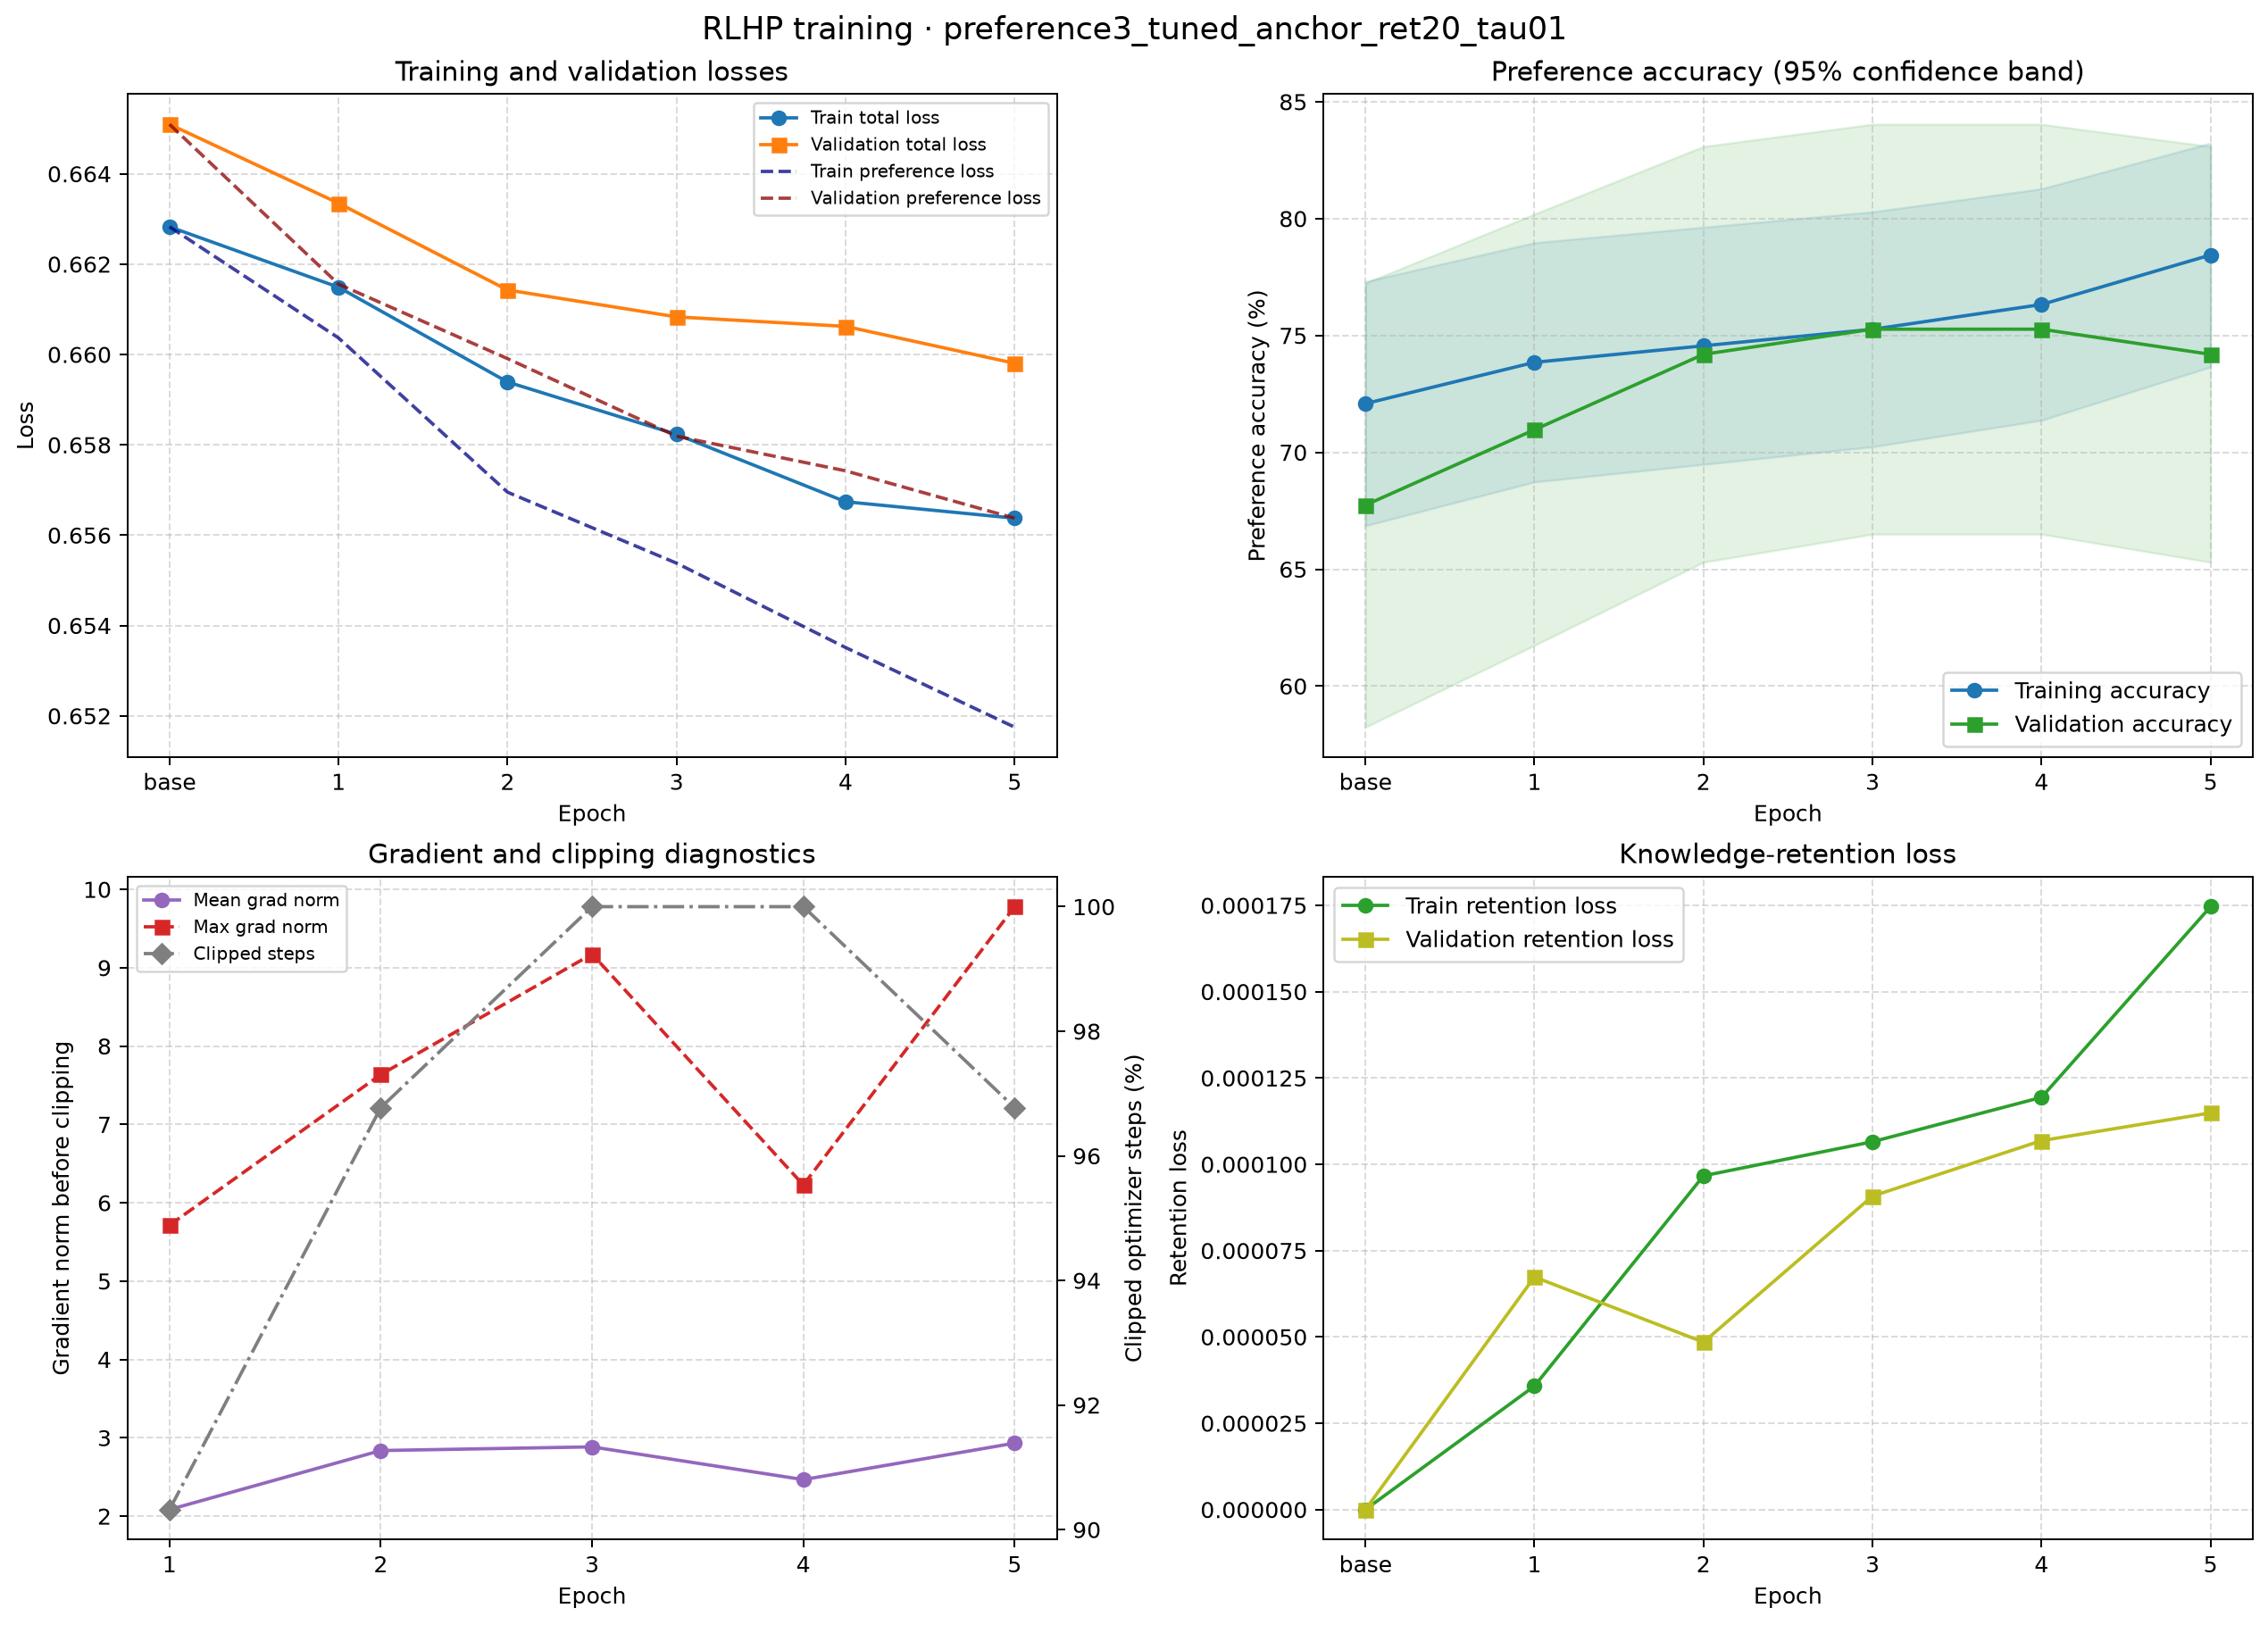
\includegraphics[width=\columnwidth]{figures/training_curves.png}
    \caption{\textbf{Preference learning diagnostics.} Four-panel training dynamics during Full RLHP fine-tuning across epochs: (top-left) total and preference losses, (top-right) strong-preference accuracy with 95\% confidence bands, (bottom-left) gradient norm and step-clipping fractions, and (bottom-right) masked knowledge-retention loss.}
    \label{fig:training_diagnostics}
\end{figure}

Figure~\ref{fig:training_diagnostics} displays the four-panel optimization diagnostics tracking Full RLHP fine-tuning across epochs.

\paragraph{Loss trajectories.}
Training preference loss decreases monotonically from $0.6604$ to $0.6517$, while validation preference loss decreases in tandem from $0.6651$ to $0.6564$, mirroring the smooth descent of the total objective. \textit{This steady downward trend confirms stable convergence without overfitting the small preference dataset.}

\paragraph{Preference accuracy.}
Strong-preference classification accuracy improves steadily from $73.85\%$ to $78.45\%$ on training and from $67.74\%$ to $74.19\%$ on validation, with narrow $95\%$ binomial confidence intervals. \textit{This gain verifies that the model successfully internalizes human preferences and generalizes to unseen validation candidate pairs.}

\paragraph{Gradient and clipping stability.}
Mean gradient norms remain bounded between $2.08$ and $2.84$ before clipping, with gradient clipping at norm $1.0$ active on $90.3\%\text{--}96.8\%$ of steps. \textit{This regularized profile ensures smooth and stable gradient propagation into the relation projection layers.}

\paragraph{Retention loss dynamics.}
The bottom-right panel tracks the masked KL retention loss on unlabelled predicates. The retention loss experiences a very slight upward progression, rising from $0.0$ to $3.58\times 10^{-5}$ in epoch 1 and reaching $1.15\times 10^{-4}$ on validation at epoch 5. This minor increase is theoretically expected: adjusting the relation projection head $\phi_{\mathrm{proj}}$ to accommodate preference targets inevitably induces subtle, microscopic shifts in the background probability mass allocated to the remaining $55$ non-target categories. \textit{Because this retention loss remains strictly constrained below $1.2\times 10^{-4}$ (orders of magnitude lower than the unconstrained explosion of $>0.04$ observed in preference-only training), it confirms that baseline semantics across unqueried predicates are rigorously preserved.}

\subsection{Quantitative PSG Test Results}
\label{sec:quant_results}

% Table 2 declared inside Section 5.3 as wide float
\begin{table*}[t]
\centering
\small
\caption{\textbf{SGDet evaluation on PSG test benchmark ($2,177$ images).} Comparison between the baseline YOLO12m-REACT++ and the Full RLHP model. Values are percentages (\%). Detection bbox mAP remains strictly invariant ($56.57\%$) due to the frozen Stage~1 detector.}
\label{tab:main_results}
\setlength{\tabcolsep}{4.5pt}
\resizebox{\textwidth}{!}{%
\begin{tabular}{lcccccccccc}
\toprule
\multirow{2}{*}{\textbf{Model}} & \multicolumn{3}{c}{\textbf{Mean Recall (mR)}} & \multicolumn{3}{c}{\textbf{Recall (R)}} & \multicolumn{3}{c}{\textbf{F1 Score}} & \textbf{Detection} \\
\cmidrule(lr){2-4} \cmidrule(lr){5-7} \cmidrule(lr){8-10} \cmidrule(lr){11-11}
& \textbf{@20} & \textbf{@50} & \textbf{@100} & \textbf{@20} & \textbf{@50} & \textbf{@100} & \textbf{@20} & \textbf{@50} & \textbf{@100} & \textbf{bbox mAP} \\
\midrule
Baseline YOLO12m-REACT++ & 23.28 & 26.37 & 28.28 & \textbf{32.63} & \textbf{38.25} & \textbf{41.45} & 27.17 & 31.22 & 33.62 & \textbf{56.57} \\
Full RLHP & \textbf{23.57} & \textbf{26.95} & \textbf{28.69} & 32.43 & 38.14 & 41.33 & \textbf{27.30} & \textbf{31.58} & \textbf{33.87} & \textbf{56.57} \\
\midrule
Absolute change & +0.30 & +0.57 & +0.41 & -0.20 & -0.11 & -0.12 & +0.13 & +0.36 & +0.24 & 0.00 \\
Relative change & +1.27\% & +2.18\% & +1.43\% & -0.62\% & -0.29\% & -0.29\% & +0.48\% & +1.16\% & +0.73\% & 0.00\% \\
\bottomrule
\end{tabular}%
}
\end{table*}

Table~\ref{tab:main_results} evaluates the baseline YOLO12m-REACT++ model against the aligned Full RLHP checkpoint on the full PSG test benchmark ($2,177$ images).

\paragraph{Macro relation quality.}
The benchmark results confirm the intended tradeoff: macro relation quality improves consistently across all evaluation cutoffs. Specifically, SGDet Mean Recall improves from $23.28\%$ to $23.57\%$ ($+0.30$ points, $+1.27\%$) at $K=20$, from $26.37\%$ to $26.95\%$ ($+0.57$ points, $+2.18\%$) at $K=50$, and from $28.28\%$ to $28.69\%$ ($+0.41$ points, $+1.43\%$) at $K=100$. Balanced F1 scores also improve monotonically across all cutoffs (F1@20: $+0.13$, F1@50: $+0.36$, F1@100: $+0.24$).

\paragraph{Instance recall and localization invariance.}
Standard instance-level Recall experiences only a negligible downward adjustment ($-0.11$ points on R@50, $-0.12$ points on R@100), which represents the standard and expected statistical shift when probability mass is redistributed away from ultra-dominant head relations toward informative medium and tail categories. Crucially, object detection bbox mAP remains strictly invariant at $56.57\%$, validating that preference optimization is strictly confined to the Stage~2 relation head without altering Stage~1 object proposals.

% Figure 4 declared inside Section 5.3 as single column
\begin{figure}[t]
    \centering
    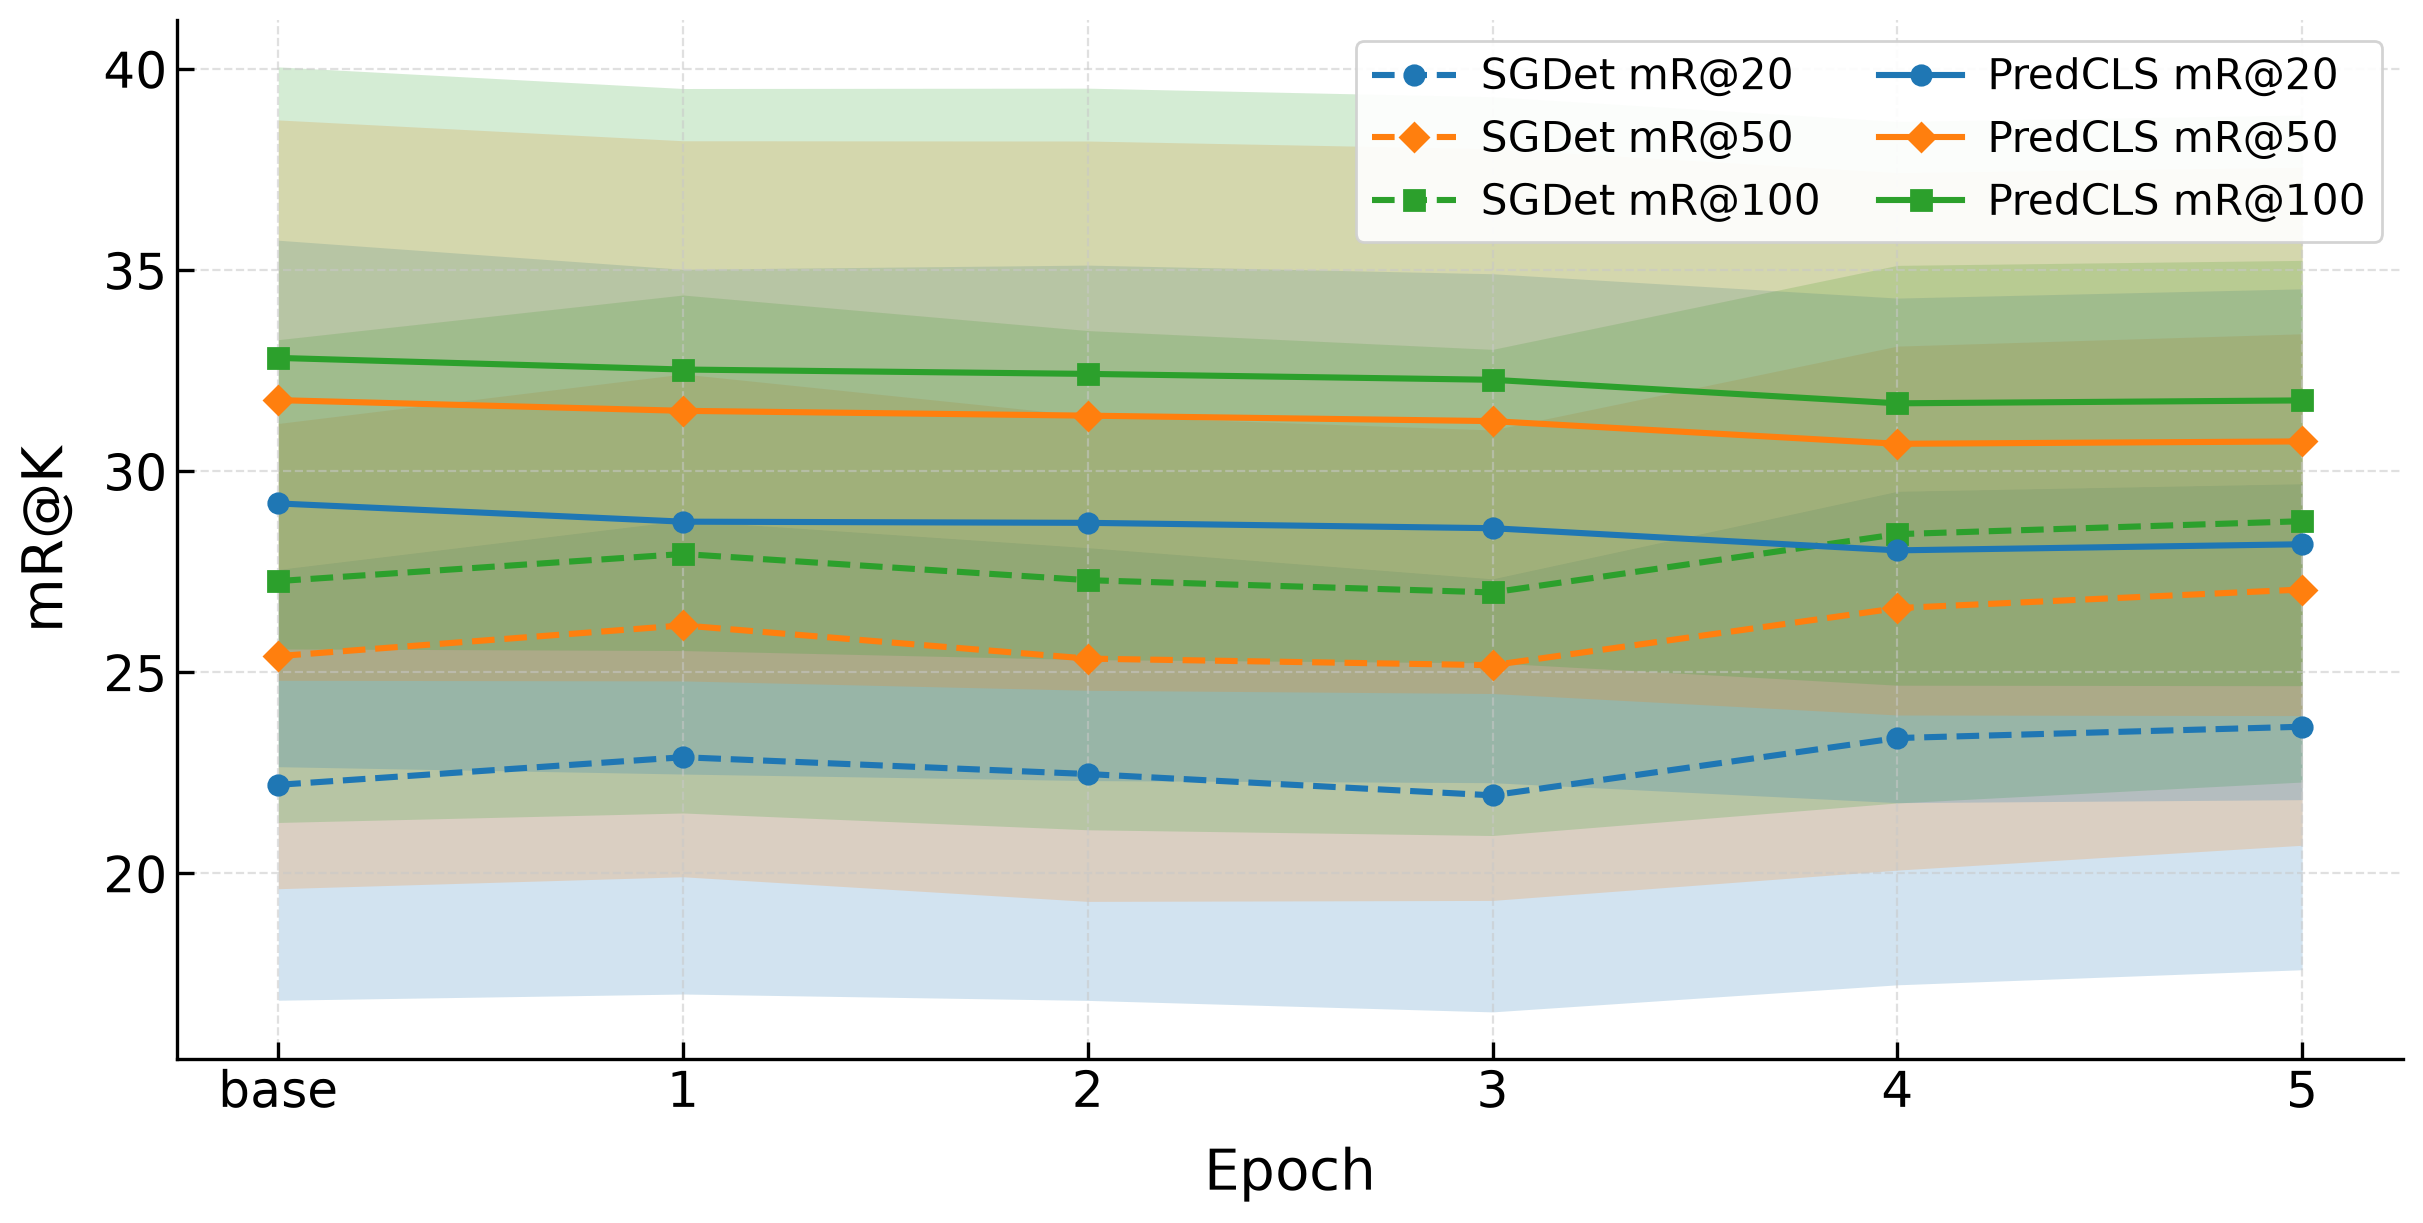
\includegraphics[width=\columnwidth]{figures/sgg_epochs_mR_curve.png}
    \caption{\textbf{PSG test mR@K over training epochs.} Macro recall trajectories across epochs demonstrate consistent test transfer and stabilization under the combined Full RLHP objective.}
    \label{fig:mr_epochs_curve}
\end{figure}

Figure~\ref{fig:mr_epochs_curve} details the PSG test macro recall trajectories across training epochs. Under the Full RLHP objective, test mR@20, mR@50, and mR@100 increase consistently as training progresses, verifying that optimization improvements on the preference set translate directly into macro-recall gains on test scene graphs without intermediate regression or instability.

\paragraph{Calibration and transfer stability.}
The epoch-wise tracking in Figure~\ref{fig:mr_epochs_curve} highlights that the relation projection head $\phi_{\mathrm{proj}}$ undergoes monotonic refinement rather than erratic oscillation. The synchronized progression across all three $K$ thresholds indicates that the learned human preferences act as a generalizable semantic inductive bias, improving rank ordering for top candidate relations without corrupting the broader predicate retrieval list.

\subsection{Loss Ablation Study}
\label{sec:ablation_retention}

% Table 3 declared inside Section 5.4 as wide float
\begin{table*}[t]
\centering
\small
\caption{\textbf{Loss ablation on PSG SGDet.} Values are candidate percentages from matched baseline/candidate evaluations on PSG test ($2,177$ images). $\Delta$ metrics ($\Delta$mR@50, $\Delta$F1@50, $\Delta$R@50) denote absolute changes relative to the matched baseline in each setting. Full RLHP is the only configuration that achieves positive gains across macro recall and F1 while maintaining stability.}
\label{tab:ablation}
\setlength{\tabcolsep}{3.5pt}
\resizebox{\textwidth}{!}{%
\begin{tabular}{lcccccccccccc}
\toprule
\multirow{2}{*}{\textbf{Configuration}} & \multicolumn{3}{c}{\textbf{Mean Recall (mR)}} & \multicolumn{3}{c}{\textbf{Recall (R)}} & \multicolumn{3}{c}{\textbf{F1 Score}} & \multicolumn{3}{c}{\textbf{Changes vs. Baseline}} \\
\cmidrule(lr){2-4} \cmidrule(lr){5-7} \cmidrule(lr){8-10} \cmidrule(lr){11-13}
& \textbf{@20} & \textbf{@50} & \textbf{@100} & \textbf{@20} & \textbf{@50} & \textbf{@100} & \textbf{@20} & \textbf{@50} & \textbf{@100} & \textbf{$\Delta$mR@50} & \textbf{$\Delta$F1@50} & \textbf{$\Delta$R@50} \\
\midrule
Preference only & 18.92 & 21.21 & 22.57 & 30.59 & 35.82 & 38.72 & 23.38 & 26.64 & 28.52 & -5.09 & -4.47 & -2.27 \\
Preference + prototype anchor & 21.24 & 24.51 & 26.18 & 31.77 & 37.31 & 40.35 & 25.46 & 29.58 & 31.76 & -0.86 & -0.89 & -0.86 \\
Preference + KL retention & 22.93 & 26.21 & 27.88 & 31.86 & 37.56 & 40.70 & 26.67 & 30.87 & 33.09 & -0.84 & -0.73 & -0.46 \\
\textbf{Full RLHP (Tuned)} & \textbf{23.57} & \textbf{26.95} & \textbf{28.69} & \textbf{32.43} & \textbf{38.14} & \textbf{41.33} & \textbf{27.30} & \textbf{31.58} & \textbf{33.87} & \textbf{+0.57} & \textbf{+0.36} & \textbf{-0.11} \\
\bottomrule
\end{tabular}%
}
\end{table*}

Table~\ref{tab:ablation} synthesizes multi-metric evaluations across all four loss configurations on the PSG test benchmark ($2,177$ images). Evaluating performance primarily through the macro-recall ceiling, \textbf{mR@100}, demonstrates the critical necessity of joint regularization: unconstrained pairwise supervision (\textit{Preference only}) achieves high validation preference fit ($82.8\%$) but catastrophically degrades test mR@100 to $22.57\%$ (a $-5.71$ point drop vs. baseline $28.28\%$). Single-loss variants partially recover but still lag baseline performance ($26.18\%$ for prototype anchor only and $27.88\%$ for KL retention only).

In contrast, the unified \textbf{Full RLHP} configuration is the sole model achieving positive transfer, setting a new peak of \textbf{$28.69\%$ mR@100} ($+0.41$ points over baseline, outperforming pure preference by $+6.12$ points). Furthermore, Full RLHP exhibits uniform superiority across all remaining evaluated metrics: leading macro recall at lower cutoffs (\textbf{mR@20 = $23.57\%$}, \textbf{mR@50 = $26.95\%$}), dominating balanced harmonic scores (\textbf{F1@20 = $27.30\%$}, \textbf{F1@50 = $31.58\%$}, \textbf{F1@100 = $33.87\%$}), and preserving standard instance recall (\textbf{R@20 = $32.43\%$}, \textbf{R@50 = $38.14\%$}, \textbf{R@100 = $41.33\%$}, avoiding the $-2.61$ point collapse of pure preference). This multi-metric dominance verifies that prototype anchoring and masked KL retention provide indispensable, synergistic safeguards that prevent semantic drift while maximizing preference transfer.

\paragraph{Synergy between retention and anchoring.}
The ablation results in Table~\ref{tab:ablation} reveal strong synergy between probability distribution retention ($\mathcal{L}_{\mathrm{KL}}$) and prototype embedding anchoring ($\mathcal{L}_{\mathrm{proto}}$). While KL retention preserves the local probability geometry over the $55$ unlabelled classes for each relation instance, prototype anchoring maintains the global metric coordinate frame of the entire predicate codebook. Applying either mechanism in isolation is insufficient to prevent test regression (mR@50 remains negative at $-0.84$ and $-0.86$ respectively). Only when both constraints are jointly active does the projection head find an optimal subspace that absorbs human preferences while fully protecting baseline visual relation knowledge.

\subsection{Analysis of Catastrophic Semantic Drift}
\label{sec:semantic_drift}

% Figure 5 declared inside Section 5.5 as single-column figure
\begin{figure}[t]
    \centering
    \begin{subfigure}[b]{0.74\columnwidth}
        \centering
        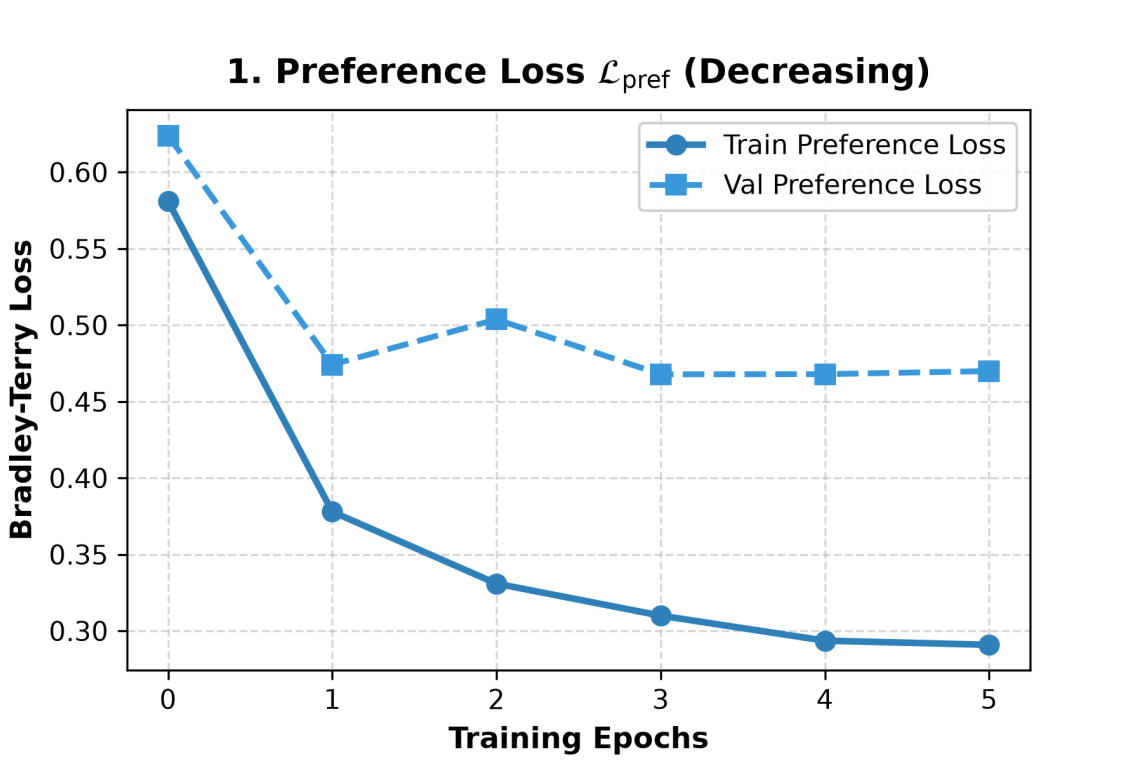
\includegraphics[width=\linewidth]{figures/retention_drift_p1.png}
        \caption{Loss trajectories \& accuracy}
        \label{fig:drift_p1}
    \end{subfigure}
    \vspace{1mm}
    \begin{subfigure}[b]{0.74\columnwidth}
        \centering
        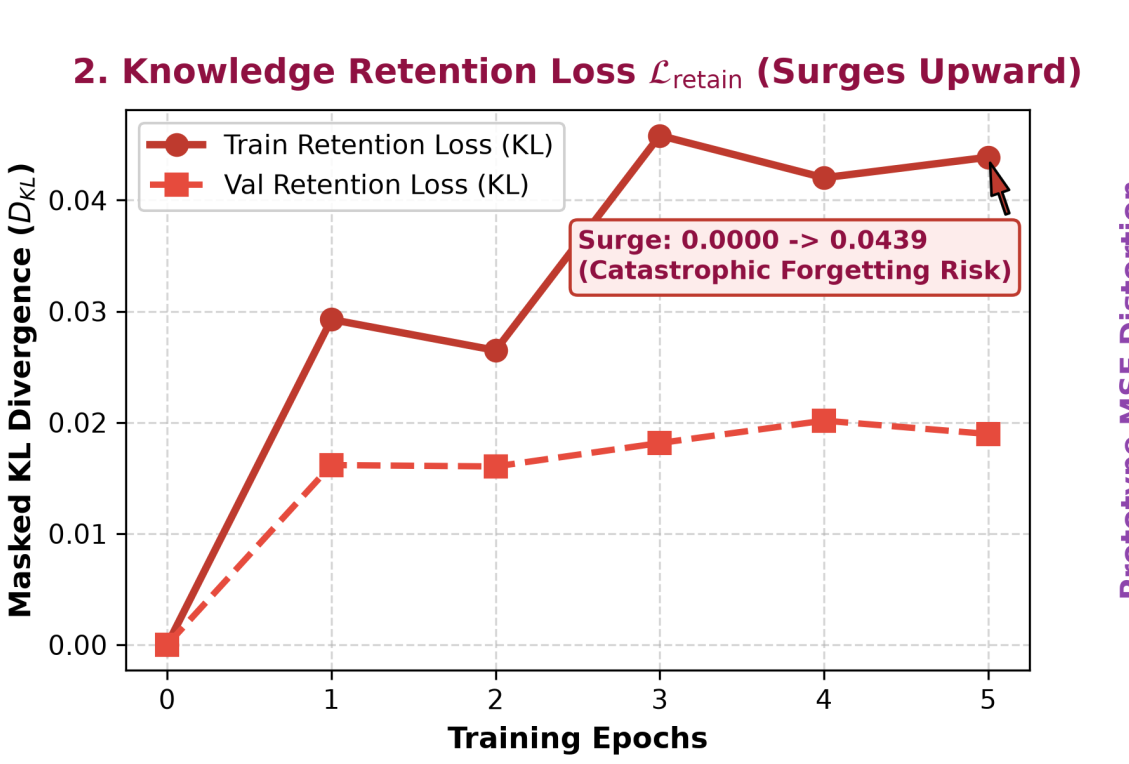
\includegraphics[width=\linewidth]{figures/retention_drift_p2.png}
        \caption{Masked KL divergence \& prototype drift}
        \label{fig:drift_p2}
    \end{subfigure}
    \vspace{1mm}
    \begin{subfigure}[b]{0.74\columnwidth}
        \centering
        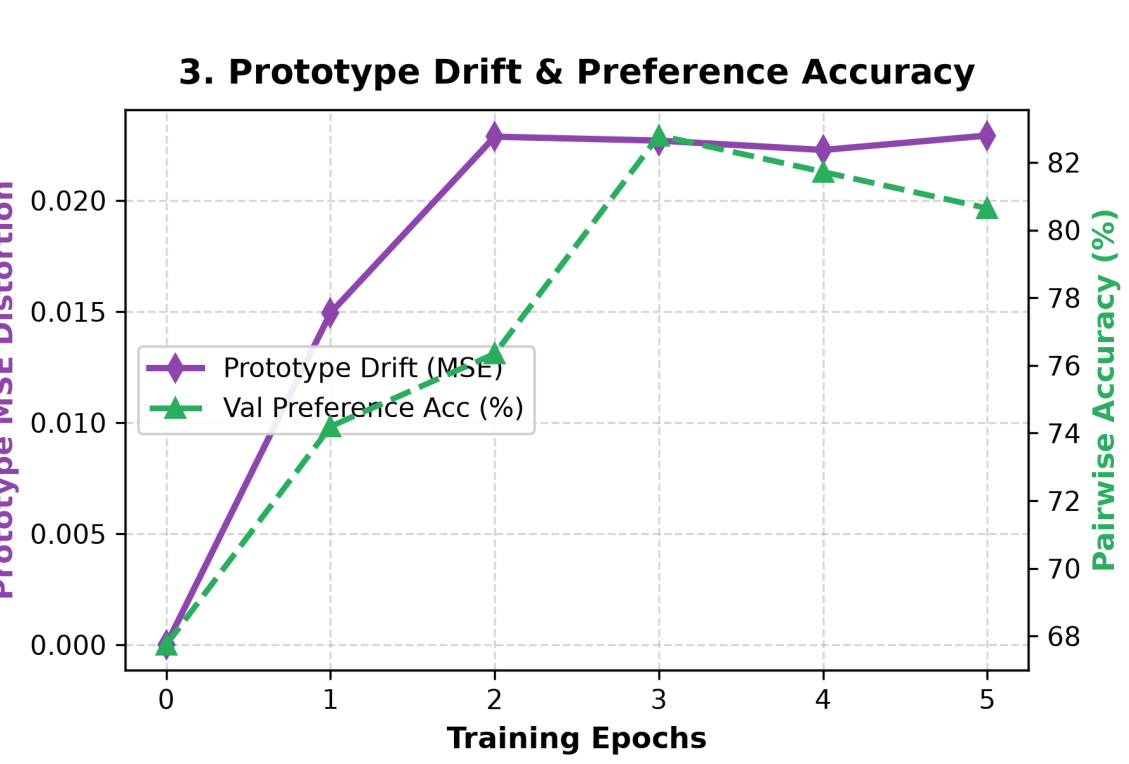
\includegraphics[width=\linewidth]{figures/retention_drift_p3.png}
        \caption{PSG test macro-recall collapse}
        \label{fig:drift_p3}
    \end{subfigure}
    \caption{\textbf{Catastrophic semantic drift under pure preference training.} Without KL retention and prototype anchoring, preference accuracy rises and Bradley-Terry loss falls, but masked KL on non-labelled classes grows sharply ($>0.04$) and prototype drift exceeds $0.02$, causing PSG test macro recall to drop precipitously.}
    \label{fig:retention_explosion}
\end{figure}

Figure~\ref{fig:retention_explosion} illustrates the internal failure mechanism of unregularized preference fine-tuning. When trained exclusively on $\mathcal{L}_{\mathrm{pref}}$, the model optimizes only the queried predicate logits, driving training preference loss down and validation accuracy up. However, the projection head $\phi_{\mathrm{proj}}$ freely distorts the rest of the embedding manifold: masked KL divergence on the $55$ unlabelled classes surges past $0.04$, while prototype drift surpasses $0.02$.

In stark contrast to the controlled diagnostics of the Full RLHP model in Figure~\ref{fig:training_diagnostics} (where masked retention loss remains strictly bounded at $\sim 1.15\times 10^{-4}$ and prototype drift is negligible at $<5.7\times 10^{-5}$), this unconstrained rotation collapses unlabelled relation boundaries, causing test mR@50 to plummet despite higher preference fit on the queried pairs. The auxiliary retention and anchoring losses in Full RLHP strictly prevent this catastrophic drift, ensuring stable test generalization.

\paragraph{Manifold distortion mechanics.}
Because the preference dataset contains pairwise comparisons for only a subset of predicates, gradient descent on $\mathcal{L}_{\mathrm{pref}}$ updates the projection matrix $\phi_{\mathrm{proj}}$ along directions that maximize separation for the annotated pairs, regardless of how other predicate prototype vectors are transformed. Without regularizing constraints, this leads to prototype crowding and subspace collapse for unannotated categories. The masked KL loss provides a sample-dependent counter-force, while the prototype anchor provides a sample-independent rigid constraint, together maintaining the semantic integrity of the entire predicate space.

\subsection{Per-Predicate and Qualitative Effects}

% Figure 6 declared inside Section 5.6 as wide float
\begin{figure*}[t]
    \centering
    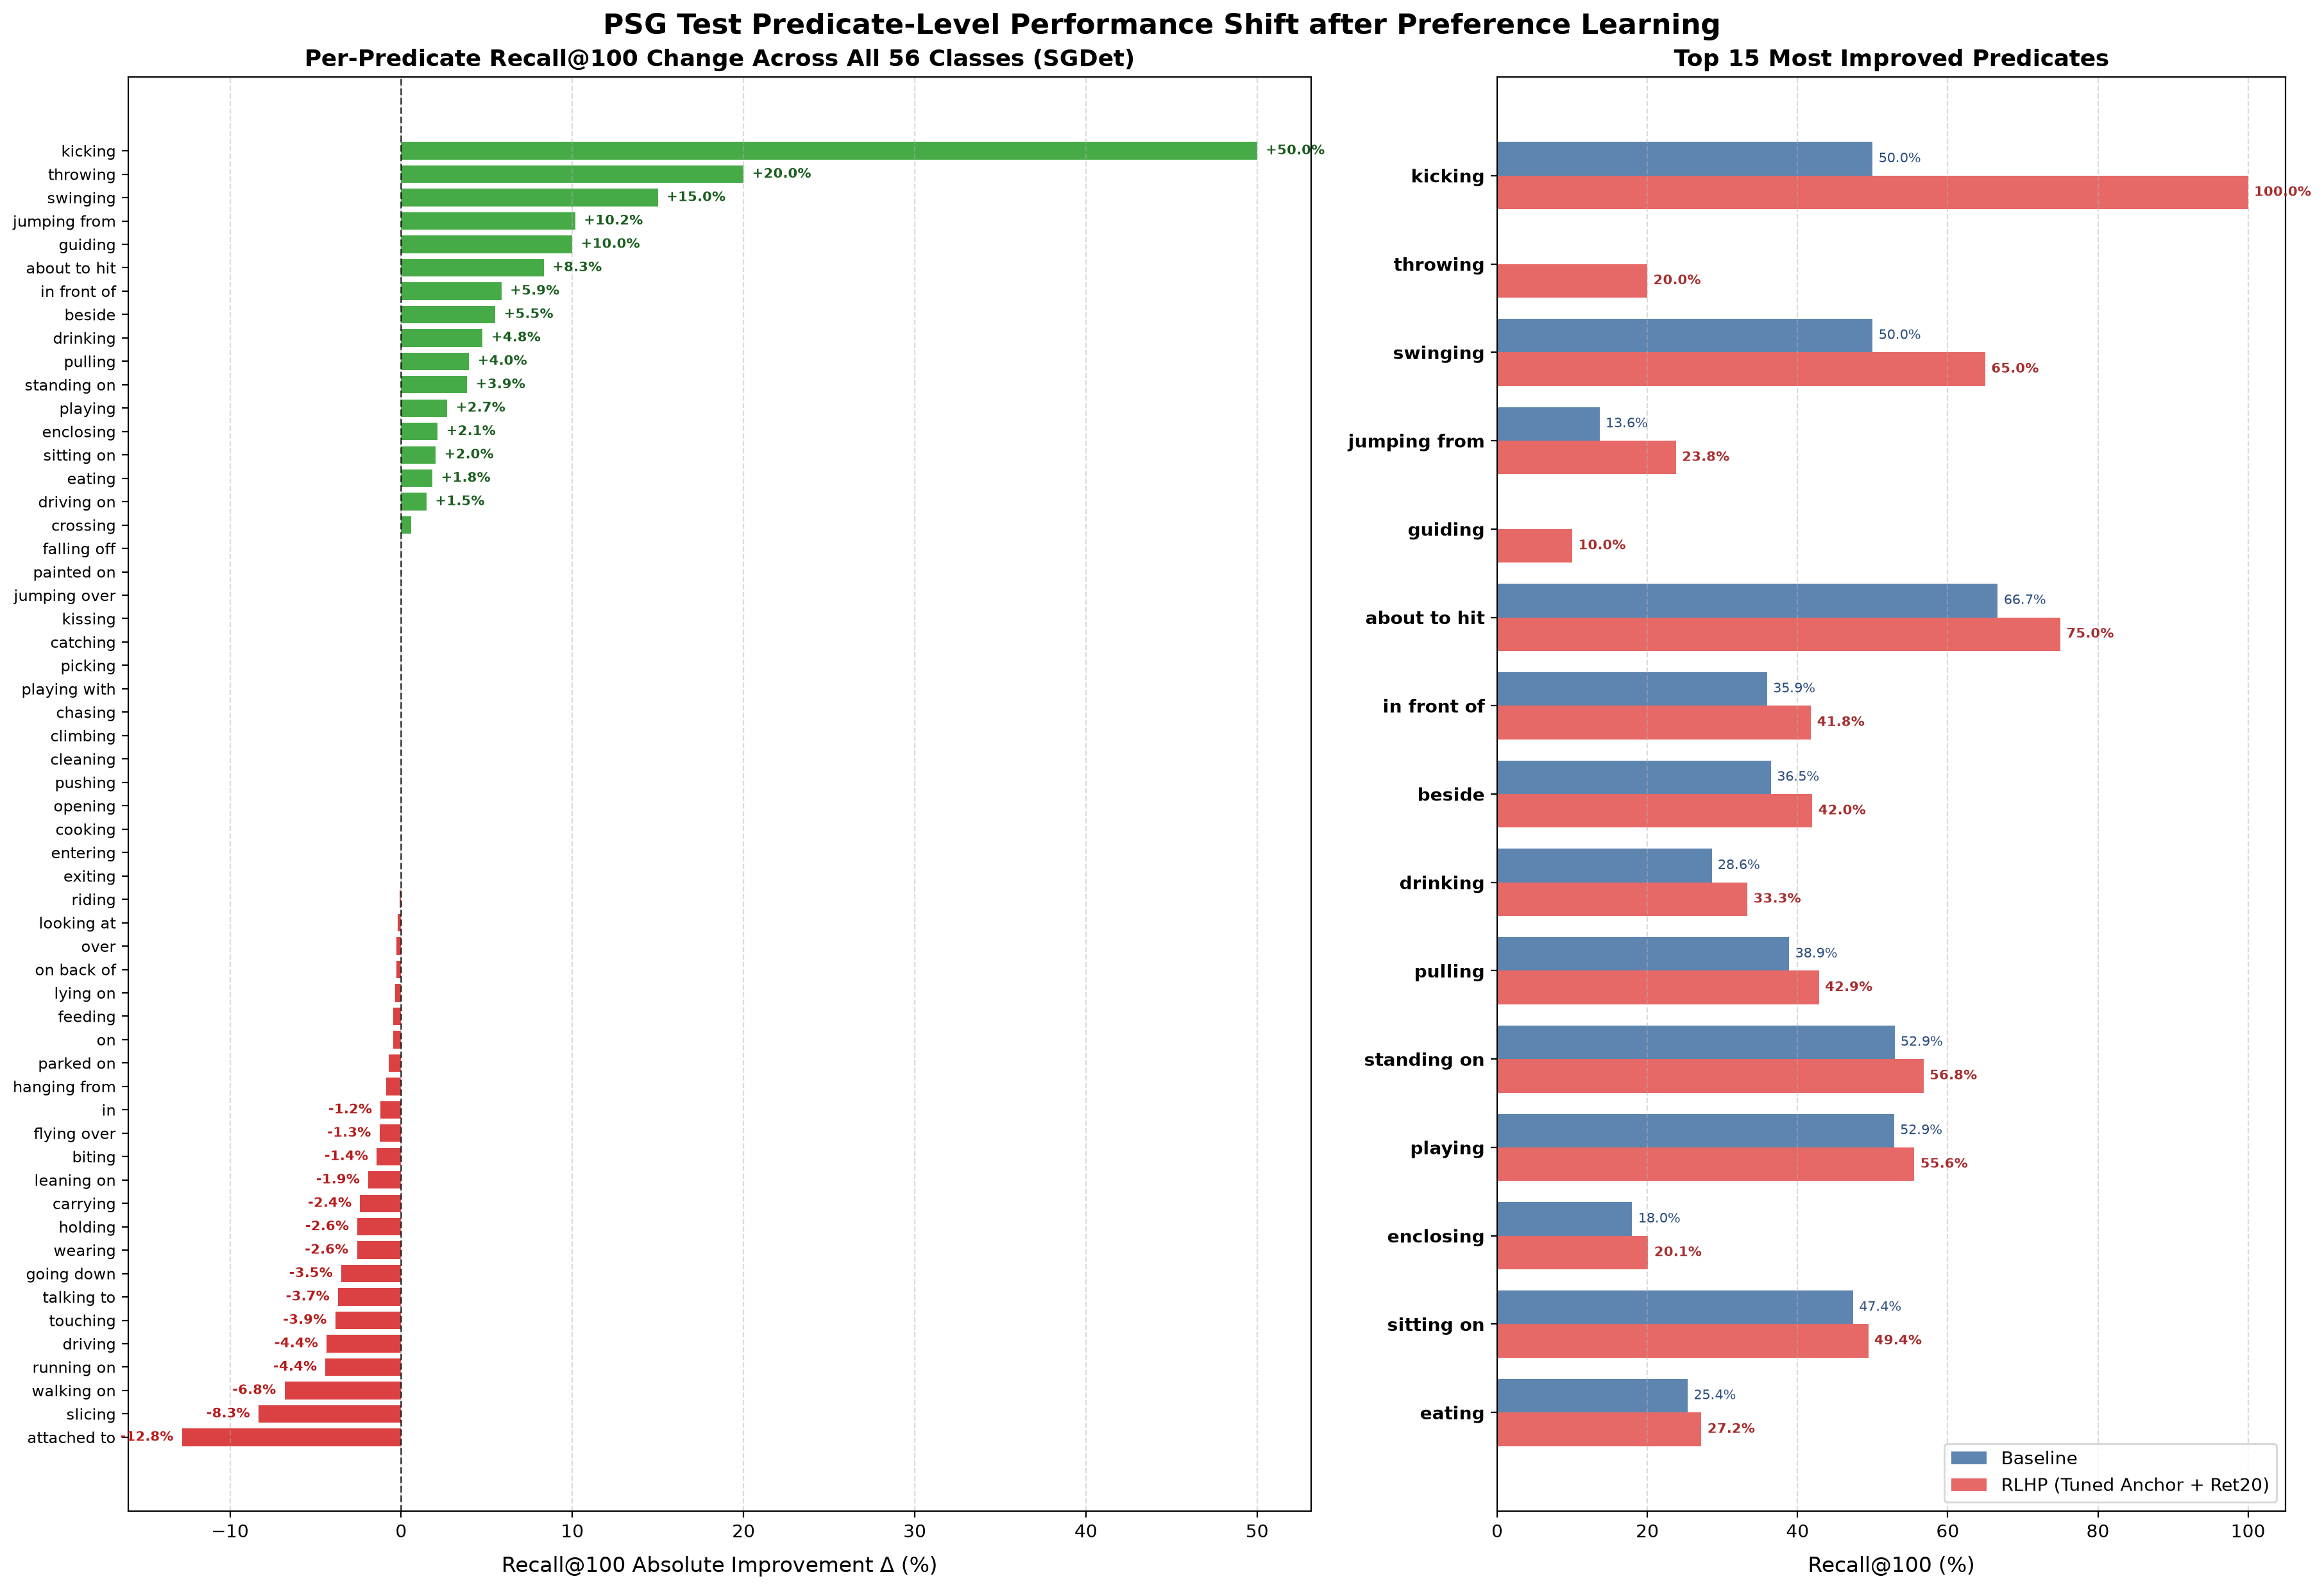
\includegraphics[width=0.58\textwidth]{figures/predicate_improvements.png}
    \caption{\textbf{Per-predicate SGDet recall shifts across all 56 foreground categories.} The largest gains occur on fine-grained spatial/action predicates such as \textit{standing on}, \textit{beside}, \textit{parked on}, and \textit{in front of}, with notable gains on discriminative tail interactions.}
    \label{fig:pred_improvements}
\end{figure*}

Figure~\ref{fig:pred_improvements} details the predicate-level recall changes across all 56 foreground relation classes under Full RLHP. The per-predicate breakdown confirms that performance gains directly align with the collected human feedback. High-frequency confusing categories---including \textit{standing on}, \textit{beside}, \textit{in front of}, and \textit{parked on}---exhibit substantial recall improvements, demonstrating that targeted pairwise supervision effectively corrects model bias on fine-grained spatial configurations.

\paragraph{Head vs. tail efficiency.}
Furthermore, several tail action predicates characterized by high semantic specificity---such as \textit{kicking}, \textit{throwing}, \textit{about to hit}, and \textit{jumping from}---show marked recall gains despite their sparse representation in the preference dataset distribution (Figure~\ref{fig:preference_distribution}). This indicates that highly discriminative, fine-grained relations exhibit high sample efficiency under human feedback: even a few targeted pairwise preference signals suffice to establish clear decision boundaries and boost predicate sensitivity without requiring extensive re-annotation. In contrast, broad geometric predicates such as \textit{on} or \textit{attached to} show calibrated adjustments, allowing more descriptive relation triplets to emerge during ranking.

% Figure 7 declared inside Section 5.6 as single column figure
\begin{figure}[t]
    \centering
    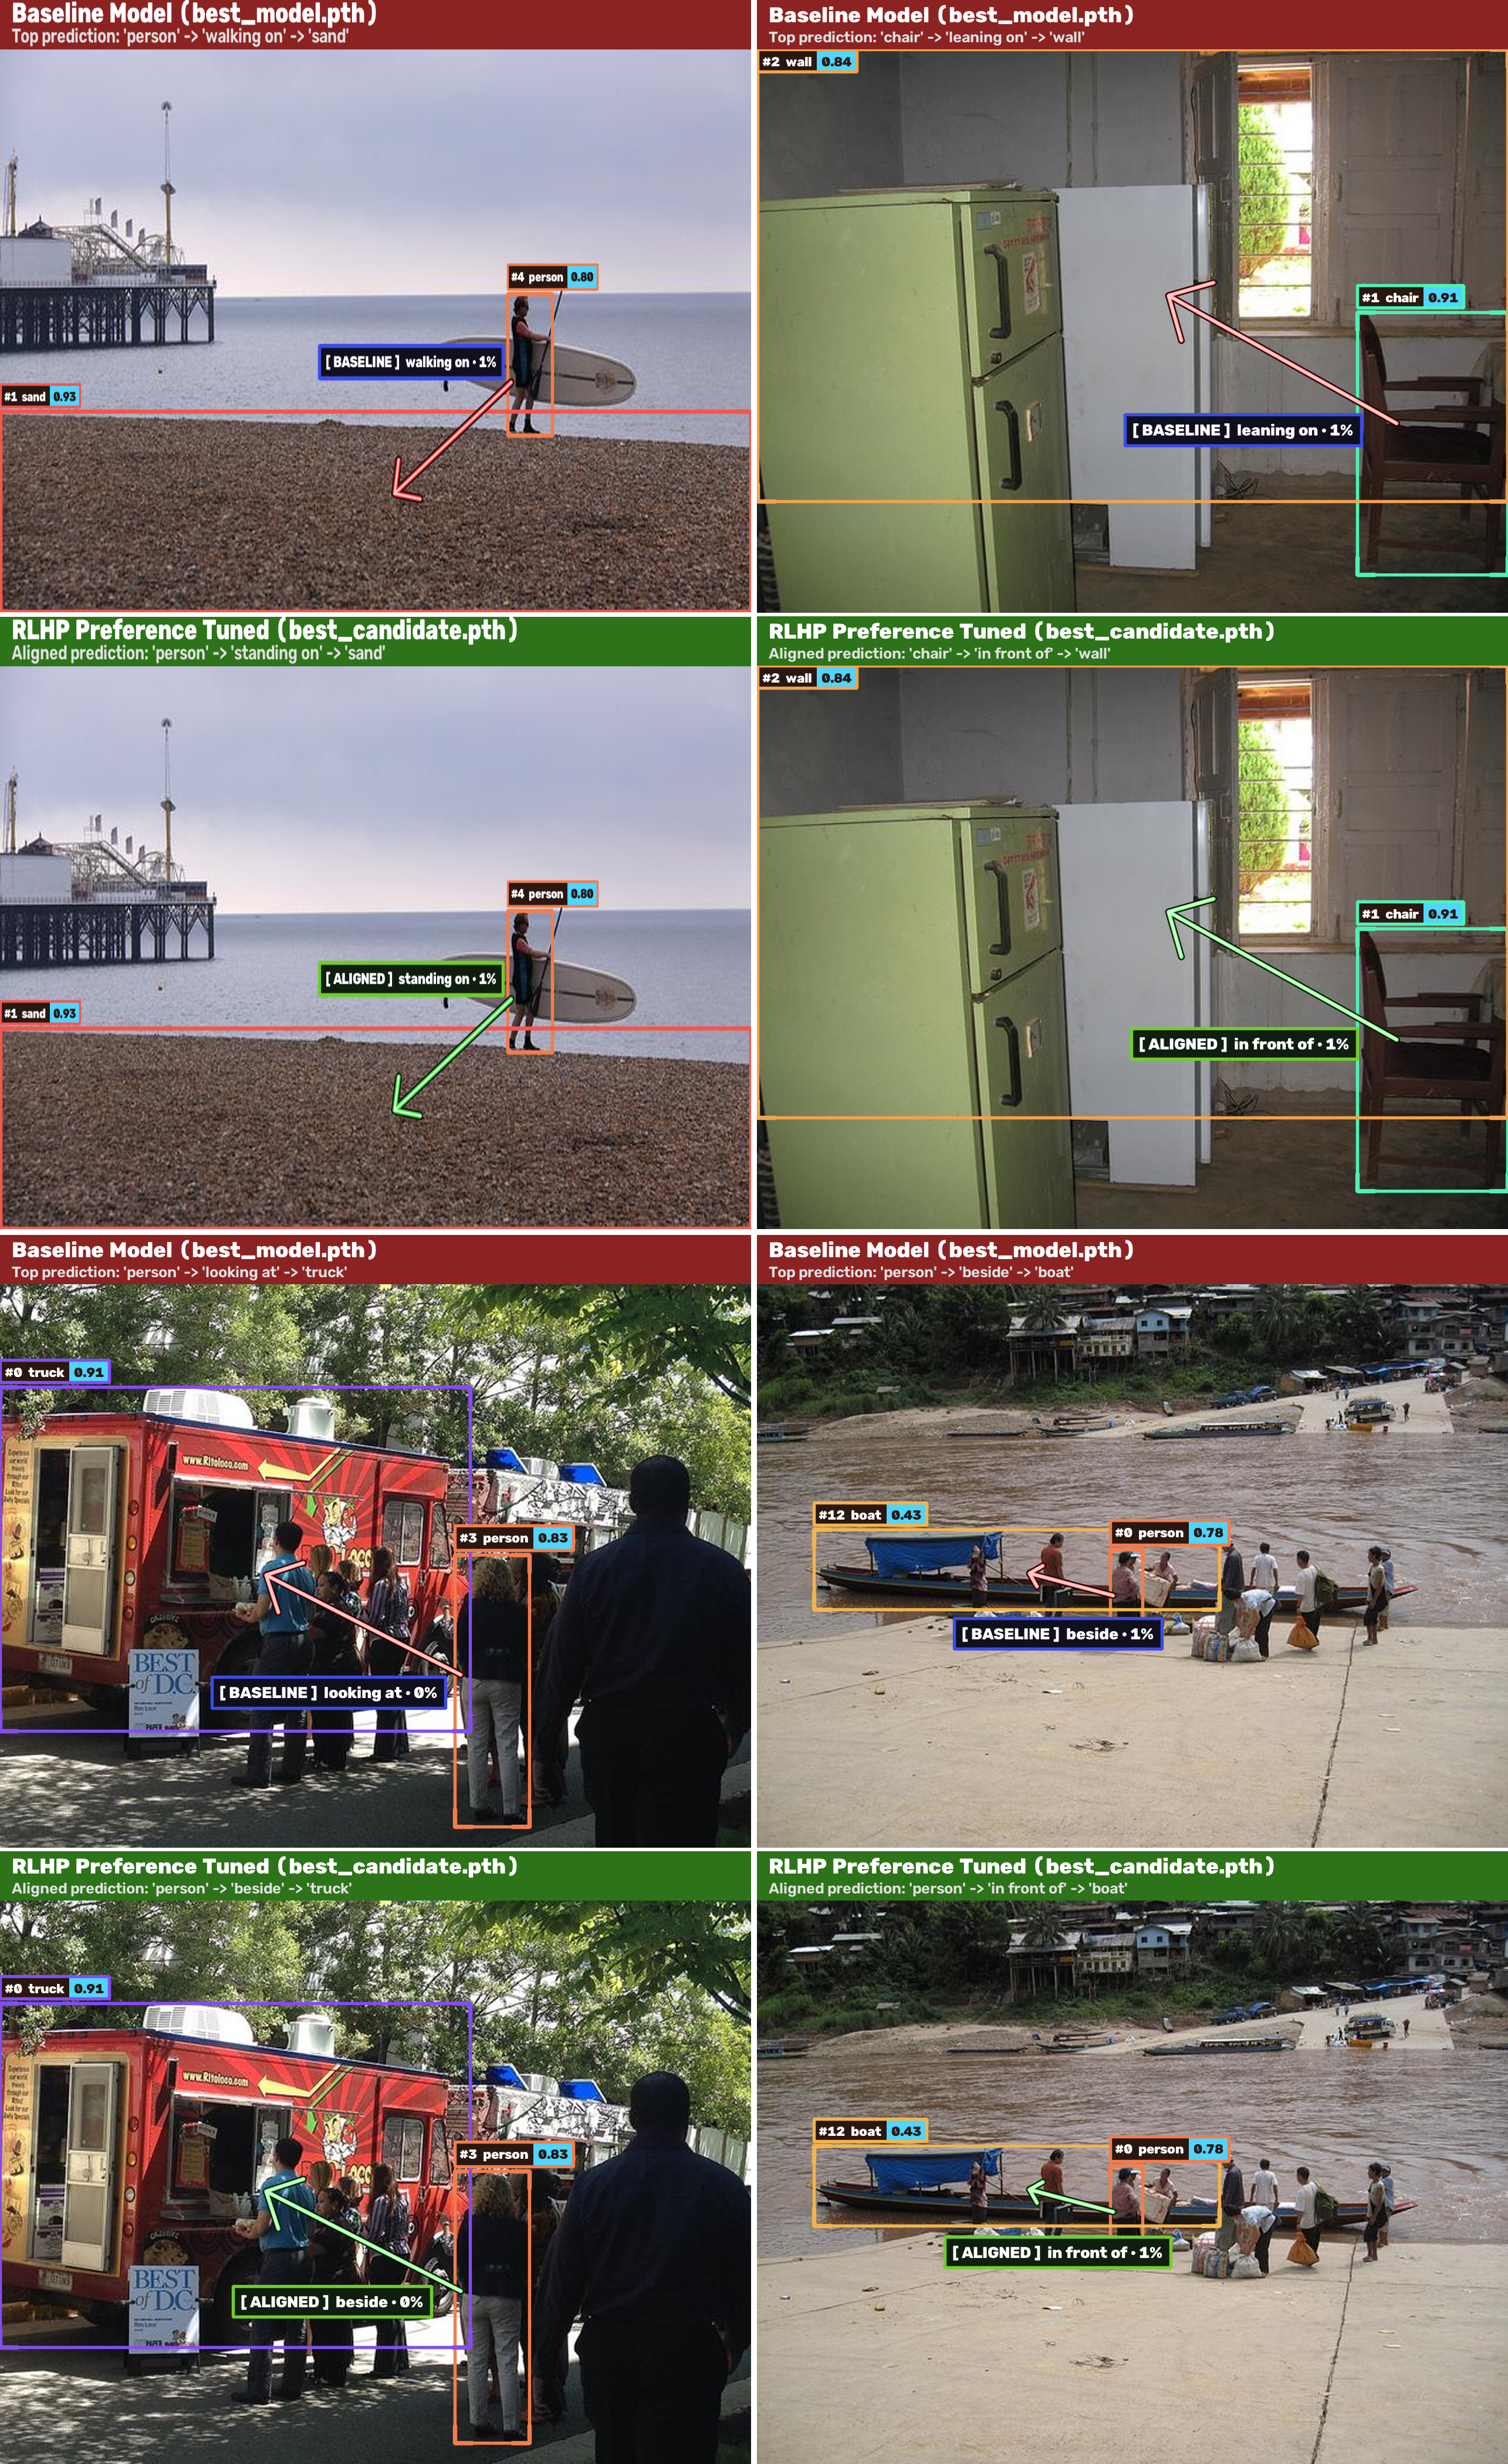
\includegraphics[width=0.62\columnwidth]{figures/qualitative_comparison_grid.png}
    \caption{\textbf{Qualitative effect of preference alignment.} The panels compare the baseline top predicate with the preference-aligned model's top predicate for the same detected subject-object pair. The aligned model often shifts generic or uncertain relations toward preference-supported predicates such as \textit{standing on}, \textit{beside}, and \textit{in front of}.}
    \label{fig:qualitative_grid}
\end{figure}

\paragraph{Qualitative visual inspection.}
Figure~\ref{fig:qualitative_grid} illustrates these qualitative transitions on test scene graphs. The preference-aligned model refines generic spatial predictions (e.g., resolving ambiguous relations into precise descriptions such as \textit{standing on}, \textit{beside}, or \textit{in front of}) while preserving correct object bounding boxes. These qualitative shifts confirm that preference learning sharpens ambiguous visual cues into specific, interpretable graph representations suitable for visual navigation.

\paragraph{Pairwise competition and inductive bias synthesis.}
The overall empirical findings validate our two-stage alignment design. Standard instance recall changes slightly downward as probability volume shifts from dominant generic classes toward informative specific categories, yielding a substantial macro-averaged gain across all evaluation cutoffs. Moreover, per-predicate shifts in Figure~\ref{fig:pred_improvements} reflect inherent pairwise competition, where prioritizing human-favored relations (e.g., \textit{beside} or \textit{standing on}) reallocates probability mass away from ambiguous counterparts (e.g., \textit{attached to} or \textit{walking on}) while preserving net macro gains. The consistency of these improvements across SGDet, PredCLS, and epoch trajectories indicates that preference learning functions as an effective, calibrated inductive bias for two-stage scene graph generation.

\section{Conclusion and Future Work}
\label{sec:conclusion}

This report presented an end-to-end human preference alignment framework for two-stage Scene Graph Generation on Panoptic Scene Graphs. By integrating human preference learning through active uncertainty-guided feedback---coupling an active uncertainty-selection GUI with a frozen Stage~1 YOLO12m detector and fine-tuning only the REACT++ relation projection layers---the framework directly enhances relation prediction accuracy on highly uncertain predicate pairs as well as relation recognition across the two-stage model in general. Crucially, ablation experiments demonstrate that pure preference optimization triggers severe representation drift; our tripartite objective---combining Bradley-Terry preference loss, masked KL retention, and prototype anchoring---rigorously safeguards the unlabelled predicate space. On the full PSG test benchmark, Full RLHP establishes a peak mR@100 of $28.69\%$ ($+0.41$ points) and improves mR@50 by $+0.57$ and F1@50 by $+0.36$ points, while keeping object detection bbox mAP strictly invariant at $56.57\%$.

\paragraph{Future work.}
For future work, the primary direction is scaling up preference data collection to a substantially larger volume while actively enforcing a balanced, comprehensive, and diverse class distribution across all relation categories. Broadening the coverage of both ambiguous head predicates and sparse tail interactions will mitigate remaining distribution skews and strengthen the model's generalization capabilities across unseen open-world environments and downstream visual navigation tasks.

\balance
{\small
\bibliographystyle{plain}
\bibliography{references}
}

\end{document}
